\documentclass[a4paper, 14pt]{article}
\usepackage[utf8]{inputenc}
\usepackage[T2A]{fontenc}
\usepackage[english,russian]{babel} 

\usepackage[left=25mm, top=20mm, right=25mm, bottom=30mm, nohead, nofoot]{geometry}
\usepackage{amsmath,amsfonts,amssymb,amsthm,extpfeil,accents}
\usepackage{fancybox,fancyhdr}
\usepackage{wasysym}
\usepackage{tikz}
\usepackage{tikz-3dplot}
\usepackage{graphicx}
\usepackage{float}
\usepackage{wrapfig}
\usetikzlibrary {decorations.markings}
\pagestyle{fancy}
\fancyhf{}
\fancyhead[R]{\href{https://t.me/empty_space1310}{Ли Любовь}}
\fancyfoot[R]{\thepage} 
\fancyhead[L]{МГТУ им. Н.Э.Баумана}
\setcounter{page}{1}
\headsep=10mm 
\usepackage{xcolor}
\usepackage{hyperref} 
\hypersetup{colorlinks=true, allcolors=[RGB]{010 090 200}}
\title{\textbf{Комплексный анализ, ФН-12, ИУ-9, 4-й семестр.\\Ответы на вопросы к экзамену\\}}
\author{  }
\date{Весна 2024}

\newextarrow{\xbigtoto}{{10}{10}{5}{5}}
   {\bigRelbar\bigRelbar{\bigtwoarrowsleft\rightarrow\rightarrow}}
\everymath{\displaystyle}

\begin{document}
\maketitle
\renewcommand{\contentsname}{Содержание}
\setcounter{page}{2}
\tableofcontents

\LARGE

\newpage 
\section{Непрерывность и дифференцируемость функций коплексного переменного, их связь. Теорема Коши-Римана. Голоморфные функции.}
\ \\
ФКП $f: \, G\subset \overline{\mathbb{C}} \rightarrow \overline{\mathbb{C}}$ \textbf{непрерывна} в точке $z_0$, если:
$$\lim\limits_{z\to z_0}f(z)=f(z_0)$$
ФКП $f(z) \,\mathbf{\mathbb{C}}$\textbf{--дифференцируема в точке $z_0$} $\Leftrightarrow$ 
\begin{enumerate}
    \item $f$ определена в окрестности точки $z_0$;
    \item $f(z_0 + \Delta z) - f(z_0) = A\Delta z + \alpha(\Delta z)\Delta z$,
\end{enumerate}
где $A \in \mathbb{C}$, $\alpha(\Delta z) \rightarrow 0$ при $\Delta z \rightarrow 0$\\[2mm]
Предел $\lim_{\Delta z \rightarrow 0} \frac{f(z_0 + \Delta z) - f(z_0)}{\Delta z}$ называют \textbf{производной ФКП $f(z)$ в точке $z_0$} и обозначают $f'(z_0)$.\\[2mm]
\textbf{Теорема (1-ый критерий $\mathbf{\mathbb{C}}$--дифференцируемости):}
\begin{center}
    ФКП $f(z)$ дифференцируема в точке $z_0$\\
    $\Leftrightarrow$\\
    $\exists$ производная $f'(z_0)$ функции $f$ в точке $z_0$, при этом $f'(z_0) = A$.
\end{center}
\begin{proof}
\ \\
''$\Rightarrow$''\\
$f'(z_0) = \lim_{\Delta z \rightarrow 0} \frac{f(z_0 + \Delta z) - f(z_0)}{\Delta z} = \lim_{\Delta z \rightarrow 0} \frac{A\Delta z + \alpha(\Delta z)\Delta z}{\Delta z} = \\
= \lim_{\Delta z \rightarrow 0} (A + \alpha(\Delta z)) = A$ $(\alpha(\Delta z) \rightarrow 0$ при $\Delta z \rightarrow 0) \Rightarrow$\\
$\Rightarrow \exists f'(z_0) = A$.\\
''$\Leftarrow$''\\
$f'(z_0) = \lim_{\Delta z \rightarrow 0} \frac{f(z_0 + \Delta z) - f(z_0)}{\Delta z}$,\\
$\alpha(\Delta z) = \frac{f(z_0 + \Delta z) - f(z_0)}{\Delta z} - f'(z_0) \rightarrow 0$ при $\Delta z \to 0 \Rightarrow$\\
$\Rightarrow f(z_0 + \Delta z) - f(z_0) = A\Delta z + \alpha(\Delta z)\Delta z$.
\end{proof}
Функция $w = f(z)$ называется \textbf{голоморфной (аналитической)} в точке $z_0 \in \mathbb{C} \Leftrightarrow f$ -- $\mathbb{C}$ -- дифференцируема в окрестности точки $z_0$.\\[2mm]
\textbf{Теорема (об условиях Коши-Римана):}\\[2mm]
Функция $f(z) = u(x, y) + iv(x, y)$, где $z = x + iy$, $\mathbb{C}$ -- дифференцируема в точке $z_0 = x_0 + iy_0$ тогда и только тогда, когда:
\begin{enumerate}
    \item Функции $u(x, y)$ и $v(x, y)$ $\mathbb{R}^2$ -- дифференцируемы в точке $M_0(x_0, y_0)$;
    \item Выполняются условия (уравнения) Коши-Римана:\\
    $\begin{cases}
        \dfrac{\partial u}{\partial x} (M_0) = \frac{\partial v}{\partial y} (M_0)\\
        \dfrac{\partial u}{\partial y} (M_0) = -\frac{\partial v}{\partial x} (M_0)
    \end{cases}$
\end{enumerate}
При этом $f'(z_0) = \frac{\partial u}{\partial x} (M_0) + i\frac{\partial v}{\partial x} (M_0) = \frac{\partial v}{\partial y} (M_0) - i\frac{\partial u}{\partial y} (M_0)$.
\begin{proof}
\ \\
''$\Rightarrow$''\\
$\Delta f(z_0, \Delta z) = A\Delta z + \gamma(\Delta z)\Delta z$, но при этом:\\
$\Delta f(z_0, \Delta z) = \Delta u(x_0, y_0, \Delta x, \Delta y) + i\Delta v(x_0, y_0, \Delta x, \Delta y) =$\\[2mm]
$ = \alpha\Delta x - \beta\Delta y + i(\alpha\Delta y + \beta\Delta x) + \gamma(\Delta z)\Delta z \Rightarrow$\\[2mm]
$\Rightarrow
\begin{cases}
    \Delta u = \alpha\Delta x - \beta\Delta y + Re(\gamma(\Delta z)\Delta z)\\
    \Delta v = \alpha\Delta y + \beta\Delta x + Im(\gamma(\Delta z)\Delta z),
\end{cases}$\\
где $\frac{\gamma(\Delta z)\Delta z}{|\Delta z|} \rightarrow 0$ при $\Delta z \rightarrow 0 \ ((\Delta x, \Delta y) \rightarrow 0)$, так как $\gamma(\Delta z) \rightarrow 0$, а $\frac{\Delta z}{|\Delta z|}$ -- ограничена при $\Delta z \rightarrow 0 \Rightarrow$\\
$\begin{cases}
    Re(\gamma(\Delta z)\Delta z) = o(|\Delta z|)\\
    Im(\gamma(\Delta z)\Delta z) = o(|\Delta z|)
\end{cases}$
$\Rightarrow$ 1);\\
$\begin{cases}
    \Delta u = u'_x\Delta x + u'_y\Delta y + o(|\Delta z|)\\
    \Delta v = v'_x\Delta x + v'_y\Delta y + o(|\Delta z|)
\end{cases} \Rightarrow$\\
$\Rightarrow
\begin{cases}
    u'_x = \alpha = v'_y\\
    u'_y = -\beta = -v'_x
\end{cases} \Rightarrow 2)$\\
Тогда $f'_z = \alpha + i\beta \Rightarrow$
$\Rightarrow f'(z_0) = \frac{\partial u}{\partial x} (M_0) + i\frac{\partial v}{\partial x} (M_0) = \frac{\partial v}{\partial y} (M_0) - i\frac{\partial u}{\partial y} (M_0)$\\[2mm]
``$\Leftarrow:$''
Аналогично
\end{proof}

\newpage
\section{Геометрический смысл комплексной производной. Конформные отображения,
связь конформности и дифференцируемости, примеры.}

Пусть задана кривая $z = z(t) = x(t) + iy(t)$, имеющая касательную в точке $t_0$ c направляющим вектором $\xi = x'(t_0) + iy'(t_0)$.
Назовем $\xi$ касательным вектором в точке $t_0$ к кривой $z$.

\begin{samepage}
\textbf{Теорема (геометрический смысл комплексной производной):}
\begin{enumerate}
  \item Любая голоморфная в т. $z_0 = z(t_0)$ функция f определяет линейное отображение касательных касательных векторов $\eta = f'(z_0)\xi$, где $\eta$ -- образ касательного вектора $\xi$, являющийся касательным вектором к кривой $f(z)$ в точке $f(z_0)$.
  \item Это отображение касательных векторов состоит в растяжении с коэффициентом $|f'(z_0)|$ и повороте на угол $arg f'(z_0)$.
\end{enumerate}
\end{samepage}

$\square$
а) По правилу дифференцирования сложной функции (в смысле $\mathbb{R}^2$)
$$\eta = \frac{df(z(t))}{dt} (t_0) = f'(z(t_0))z'(t_0) = f'(z_0)\xi$$

б) $|\eta| = |f'(z_0)| \cdot |\eta|$ -- растяжение с коэффициентом $|f'(z_0)|$; 

$arg \eta = arg f'(z_0) + arg \xi \pm 2\pi$ -- поворот на угол $arg f'(z_0)$.

\hfill$\blacksquare$

Отображение $F$ называется \textbf{конформным} в точке $M_0(x_0,y_0)$ тогда и только тогда, когда касательное отображение в точке $M_0$ сохраняет углы.

Отображение $F$ называется \textbf{конформным} в области $U \subset \mathbb{R}^2$ тогда и только тогда, когда оно конформно в любой из точек $U$.

$U\subset \mathbb{C}$, $H(U)$ -- множество голоморфных в $U$ функций.

\textbf{Теорема (о связи конформности и диффиренцируемости):}\\
$U$ -- область в $\mathbb{C}$. Если $f\in H(U)$ и $\forall z\in U~~f'(z) \neq 0$, тогда $f$ -- конформное в $U$ отображение.

$\square$
Доказательство следует из предыдущей теоремы:\\
В каждой точке $z_0 \in U$ лин.отображение $f'(z_0)$ растигивает в $|f'(z_0)|\neq 0$ и поворачивает на угол $arg\,f'(z_0)\Rightarrow$ лин.отображение в $z_0$ сохраняет углы. 

\hfill$\blacksquare$

\textbf{Определение:} Угол между кривыми $\gamma_1$ и $\gamma_2$ в точке $\infty$ равнен углу между касательными к $\hat{\gamma}_1$ и $\hat{\gamma}_2$ в точке 0, где $\hat{\gamma}_1 = \frac{1}{\gamma_1}$ и $\hat{\gamma}_2 = \frac{1}{\gamma_2}$.

Отображение $F$ называется \textbf{конформным} в точке $\infty$ тогда и только тогда, угол между кривыми $\gamma_1$ и $\gamma_2$ в точке $\infty$ равен углу между кривыми $f(\gamma_1)$ и $f(\gamma_2)$ в точке $\infty$.

\newpage
\section{Определить дробно-линейное отображение (ДЛО). Сформулировать и доказать конформность и групповое свойство ДЛО.}


\textbf{Дробно-линейные отображения} --- это функции вида: $$w=\frac{az+b}{cz+d}, \text{где } \ \begin{vmatrix}
    a&b\\
    c&d
\end{vmatrix} \neq 0, \ a,b,c,d\in \mathbb{C}$$

Доопределим функцию выше следующим образом:$$z=-\frac{d}{c}: \ w(-\frac{d}{c}) = \infty$$
$$z = \infty: \ w(\infty) = \left[\begin{gathered}\frac{a}{c}, \ c\neq 0\\
\infty, \ c=0
\end{gathered}
\right.$$
Тогда ДЛО: $w: \overline{\mathbb{C}}\to \overline{\mathbb{C}}$


\textbf{Конформность:}

Любое ДЛО --- конформное отображение $\overline{\mathbb{C}}\to \overline{\mathbb{C}}$

\begin{proof}
    \ \\
    1) Рассмотрим точки $z_0 \neq -\frac{d}{c}, \ \infty:$
    
    Тогда $w'=\frac{a(cz+d)-(az+b)c}{(cz+d)^2} = \frac{ad-bc}{(cz+d)^2} \neq 0$

    Значит функция $w$ голоморфна в точках $z_0$ и по теореме о конформности голоморфных отображений, она конформна в этих точках $z_0$.

    2) Рассмотрим точку $z_0=-\frac{d}{c}:$ $$z\overset{L}{\longrightarrow}w=\frac{az+b}{cz+d}\overset{L_0}{\longrightarrow} \xi=\frac{1}{w}$$ $$\mathbf{-\frac{d}{c}} \ \overset{L}{\longrightarrow} \ \mathbf{\infty} \ \overset{L_0}{\longrightarrow} \ \mathbf{0}$$
    Отображение $\xi=\frac{1}{w}$ сохраняет углы, то есть $L_0$ конформно.
    Рассмотрим $L_0\circ L$ в точке $z_0=-\frac{d}{c}:$
    $$(L_0\circ L)^{'}_{|z=-\frac{c}{d}} = \frac{cb-ad}{(az+b)^2}_{|_{z=-\frac{c}{d}}} \neq 0$$
    Значит отображение $L_0\circ L$ конформно в точке $z_0=-\frac{c}{d}$\\
    $L=L_0^{-1}\circ (L_0\circ L)$ конформно, так как композиция конформных и обратное к конформному отображению конформны.

    3) Рассмотрим точку $z_0=\infty$:
    $$\xi=\frac{1}{z} \ \overset{L_0}{\longleftarrow} \ z \ \overset{L}{\longrightarrow} \ w=\frac{az+b}{cz+d}$$
    $$\mathbf{0} \ \overset{L_0}{\longleftarrow} \ \mathbf{\infty} \ \overset{L}{\longrightarrow} \ \mathbf{\frac{a}{c}}$$
    Рассмотрим отображение $L\circ L_0^{-1}$:
    $$w=\frac{a\cdot \frac{1}{\xi}+b}{c\cdot \frac{1}{\xi}+d} = \frac{b\cdot \xi+a}{d\cdot \xi +c}$$
    $$w^{'}_{|_{0}} = \frac{dc-da}{(d\cdot\xi+c)^2}_{|_{\xi=0}}\neq 0$$
    Значит отображение $L\circ L_{0}^{-1}$ конформно в точке $\xi_0 = 0$.\\
    Тогда отображение $L=(L\circ L_{0}^{-1})\circ L_0$ конформно в точке $z_0=\infty$, так как композиция конформных и обратное к конформному отображению конформны. 
\end{proof}

\textbf{Групповое свойство ДЛО:}

Совокупность всех ДЛО $\Lambda$ образует некоммутативную группу $(\Lambda; \circ)$ относительно операции композиции.

\begin{proof}
    \ \\
    0) Замкнутость:\\
    $w=\frac{az+b}{cz+d}; \ \xi=\frac{a_1w+b_1}{c_1w+d_1}$\\[2mm]
    $\xi=\frac{a_1\cdot\frac{az+b}{cz+b}+b_1}{c_1\cdot\frac{az+b}{cz+b}+d_1} =\frac{a_1(az+b)+b_1(cz+d)}{c_1(az+b)+d_1(cz+d)}=$\\
    $= \frac{(a_a+b_1c)z+a_1b+b_1d}{(c_1a+d_1c)z+c_1b+d_1d}$\\[2mm]
    Определитель $\begin{vmatrix}
        a_1a+b_1c & a_1b+b_1d\\
        c_1a+d_1c & c_1b+d_1d
    \end{vmatrix}$ не равен 0, так как иначе композиция ДЛО была бы отображением в одну точку, но композиция биекций есть биекция.\\[2mm]
    1) Ассоциативность выполняется, так как композиция отображений ассоциативна\\[2mm]
    2) Существование единицы:\\
    $E: \ w=z, \ \begin{pmatrix} a=1&b=0\\c=0&d=1\end{pmatrix}, \ det = 1\neq0$\\[2mm]
    3) Существование обратного:\\
    Пусть $L: \ w=\frac{az+b}{cz+d}$ --- ДЛО.\\
    Построим обратное:
    $$w(cz+d)=az+b$$
    $$z(wc-a)=b-dw$$
    $$L^{-1}: \ z=\frac{b-dw}{wc-a} \text{ --- ДЛО, так как } \ \begin{vmatrix}-d&b\\c&-a\end{vmatrix}=ad-bc\neq0$$ 
    4) Некоммутативность:\\
    Приведем контрпример
    $$L_1: \ w=z+a, \ L_2: \ w=\frac{1}{z}$$
    $$L_1\circ L_2: \ z \overset{L_2}{\rightarrow} w=\frac{1}{z} \overset{L_1}{\rightarrow} w = \frac{1}{z}+a$$
    $$L_2 \circ L_1: \ z \overset{L_1}{\rightarrow} w = z+a \overset{L_2}{\rightarrow} w = \frac{1}{z+a}$$
    Получили, что $L_1\circ L_2 \neq L_2 \circ L_1$
\end{proof}

\newpage
\section{Дробно-линейные функции, их геометрическая интерпретация и свойство трёх точек.}

\textbf{Дробно-линейные отображения} --- это функции вида: $$w=\frac{az+b}{cz+d}, \text{где } \ \begin{vmatrix}
    a&b\\
    c&d
\end{vmatrix} \neq 0, \ a,b,c,d\in \mathbb{C}$$

Доопределим функцию выше следующим образом:$$z=-\frac{d}{c}: \ w(-\frac{d}{c}) = \infty$$
$$z = \infty: \ w(\infty) = \left[\begin{gathered}\frac{a}{c}, \ c\neq 0\\
\infty, \ c=0
\end{gathered}
\right.$$
Тогда ДЛО: $w: \overline{\mathbb{C}}\to \overline{\mathbb{C}}$


\textbf{Геометрическая интерпретация:}
ДЛО --- взаимно-однозначное непрерывное отображение $\overline{\mathbb{C}}\to \overline{\mathbb{C}}$

\textbf{Теорема о трех точках} \\
Для любых трех различных точек $z_1, z_2, z_3$ и других трех различных точек $w_1, w_2, w_3$ 
существует единственное ДЛО $L(z): L(z_i) = w_i$

\textbf{Доказательство} \\
1) \textit{Существование} \\
Для любых 3-х точек $z_1, z_2, z_3$
существует ДЛО, отображающее их в $0, \infty, 1$ соответственно:
$$
w = \frac{z - z_1}{z - z_2}\cdot\frac{z_3 - z_2}{z_3 - z_1}
$$
Тогда рассмотрим отображения $L_1: \xi = \frac{z - z_1}{z - z_2}\cdot\frac{z_3 - z_2}{z_3 - z_1}$
и $L_2: \xi = \frac{w - w_1}{w - w_2}\cdot\frac{w_3 - w_2}{w_3 - w_1}
$. Из группового свойства ДЛО следует, что $L_2^{-1}$ -- тоже ДЛО, и композиция ДЛО -- тоже ДЛО.
Тогда получаем, что отображение $L = L_2^{-1} \circ L_1$ есть ДЛО, причем
\begin{equation}
\begin{gathered}
    \begin{pmatrix}
        z_1 \\
        z_2 \\
        z_3
    \end{pmatrix}
    \overset{L_1}{\rightarrow}
    \begin{pmatrix}
        0 \\
        \infty \\
        1
    \end{pmatrix}
    \overset{L_2^{-1}}{\rightarrow}
    \begin{pmatrix}
        w_1 \\
        w_2 \\
        w_3
    \end{pmatrix},
\end{gathered}
\end{equation}
то есть $L$ есть искомое ДЛО. \\
2) \textit{Единственность}
Пусть $\lambda$ -- ДЛО, отличное от $L$, построенного в пункте 1, удовлетворяющее условиям теоремы. \\
Рассмотрим отображение $\mu = L_2 \circ \lambda \circ L_1^{-1}$. Из группового свойства ДЛО полученное отображание -- ДЛО, причем
\begin{equation}
\begin{gathered}
    \mu: 
    \begin{pmatrix}
        0 \\
        \infty \\
        1
    \end{pmatrix}
    \rightarrow 
    \begin{pmatrix}
        0 \\
        \infty \\
        1
    \end{pmatrix}
\end{gathered}
\end{equation}
Теперь покажем, что $\mu = id$: \\
$\mu = \frac{az + b}{cz + d}$ \\ \\
a) $\mu(\infty) = \frac{a}{c} = \infty \Rightarrow c = 0$ \\ \\
b) $\mu(0) = \frac{b}{d} = 0 \Rightarrow b = 0$ \\ \\
c) $\mu(1) = \frac{a}{d} = 1 \Rightarrow a = d$ \\ \\
В итоге получаем, что $\mu(z) = z \Rightarrow \mu = id$,
то есть $L_2 \circ \lambda \circ L_1^{-1} = id \Rightarrow \lambda = L_2^{-1} \circ L_1 = L$, что и требовалось доказать.
\newpage
\section{Дробно-линейные функции, их геометрические свойства: круговое свойство и сохранение симметричности.}


\textbf{Дробно-линейные отображения} --- это функции вида: $$w=\frac{az+b}{cz+d}, \text{где } \ \begin{vmatrix}
    a&b\\
    c&d
\end{vmatrix} \neq 0, \ a,b,c,d\in \mathbb{C}$$

Доопределим функцию выше следующим образом:$$z=-\frac{d}{c}: \ w(-\frac{d}{c}) = \infty$$
$$z = \infty: \ w(\infty) = \left[\begin{gathered}\frac{a}{c}, \ c\neq 0\\
\infty, \ c=0
\end{gathered}
\right.$$
Тогда ДЛО: $w: \overline{\mathbb{C}}\to \overline{\mathbb{C}}$


\textbf{Круговое свойство ДЛО}\\
Любое ДЛО преобразует обобщенную окружность (окружность и ли прямая в $\overline{\mathbb{C}}$) в обобщенную окружность.

\begin{proof}
    \ \\
    1) случай, когда $c=0$:\\
    $L: \ w = az+b$\\
    $z \overset{L_1}{\rightarrow} z_1=az \overset{L_2}{\rightarrow}z_2=z_1+b$\\
    $L_1$ --- растяжение с поворотом: окружность перейдет в окружность, а прямая в прямую\\
    $L_2$ --- сдвиг: окружность перейдет в окружность, а прямая в прямую\\[2mm]
    2) случай, когда $c\neq 0$:\\
    $L: \ w=\frac{az+b}{cz+d}=\frac{a}{c} +\left(\frac{az+b}{cz+d}-\frac{a}{c}\right) = \frac{a}{c}+\frac{caz+bz-acz-ad}{c(cz+d)}=$\\[2mm]
    $\frac{a}{c}+\frac{bc-ad}{c(cz+d)}=\frac{a}{c}+\frac{\frac{bc-ad}{c}}{z+\frac{d}{c}}$\\[2mm]
    Обозначим $A=\frac{a}{c}, \ B=\frac{bc-ad}{c}, \ C=\frac{d}{c}:$\\[2mm]
    $L: \ w = A + \frac{B}{z+C}$\\[2mm]
    $z \overset{L_1}{\rightarrow} z_1=z+C \overset{L_2}{\rightarrow}z_2=\frac{1}{z_1} \overset{L_3}{\rightarrow}z_3=B\cdot z_2 \overset{L_4}{\rightarrow} w = A+z_3$\\[2mm]
    Отображения $L_1$ и $L_4$ --- сдвиги, $L_3$ --- растяжение с поворотом. Они переводят окружности в окружности, а прямые в прямые.\\
    Рассмотрим отображение $L_2: \ w=\frac{1}{z}$\\[2mm] 
    Общее уравнение обобщённой окружности на плоскости $xOy$:
    $$E(x^2+y^2) +F_1x + F_2 y + G=0$$
    $$E, F_1, F_2, G \in \mathbb{R}, \ (E, F_1, F_2, G) \neq (0, 0, 0, 0)$$
    Запишем это уравнение через переменную $z=x+iy$:
    $$x=\frac{z+\overline{z}}{2}, \ y=\frac{z-\overline{z}}{2i}=i\frac{\overline{z}-z}{2}$$
    $$Ez\overline{z}+F_1\frac{z+\overline{z}}{2}+F_2i\frac{\overline{z}-z}{2}+G=0$$
    $$Ez\overline{z}+Fz+\overline{F}\overline{z}+G=0,$$
    $$\text{где }F=\frac{1}{2}F_1-\frac{1}{2}iF_2 \in \mathbb{C}, \ \overline{F} = \frac{1}{2}F+\frac{1}{2}iF_2$$
    Тогда кривая, полученная в результате преобразования $L_2$ задается уравнением:
    $$E\frac{1}{z}\overline{\left(\frac{1}{z}\right)}+F\frac{1}{z}+\overline{F}\overline{\left(\frac{1}{z}\right)}+G=0|\cdot z\overline{z}$$
    $$E+F\overline{z}+\overline{F}z+Gz\overline{z}=0,$$
    что является уравнением обобщенной окружности.
    Значит отображение $L_2$ переводит обобщенную окружность в обобщенную окружность.
\end{proof}


\textbf{Свойство ДЛО сохранения симметричности}\\
Произвольное ДЛО $L$ преобразует любые точки $z$ и $z^*$, симметричные относительно обобщенной окружности $\Gamma$, в точки $L(z)$ и $L(z^*)$, симметричные относительно обобщенной окружности $L(\Gamma)$.

\begin{figure}[!ht]
    \begin{center}
    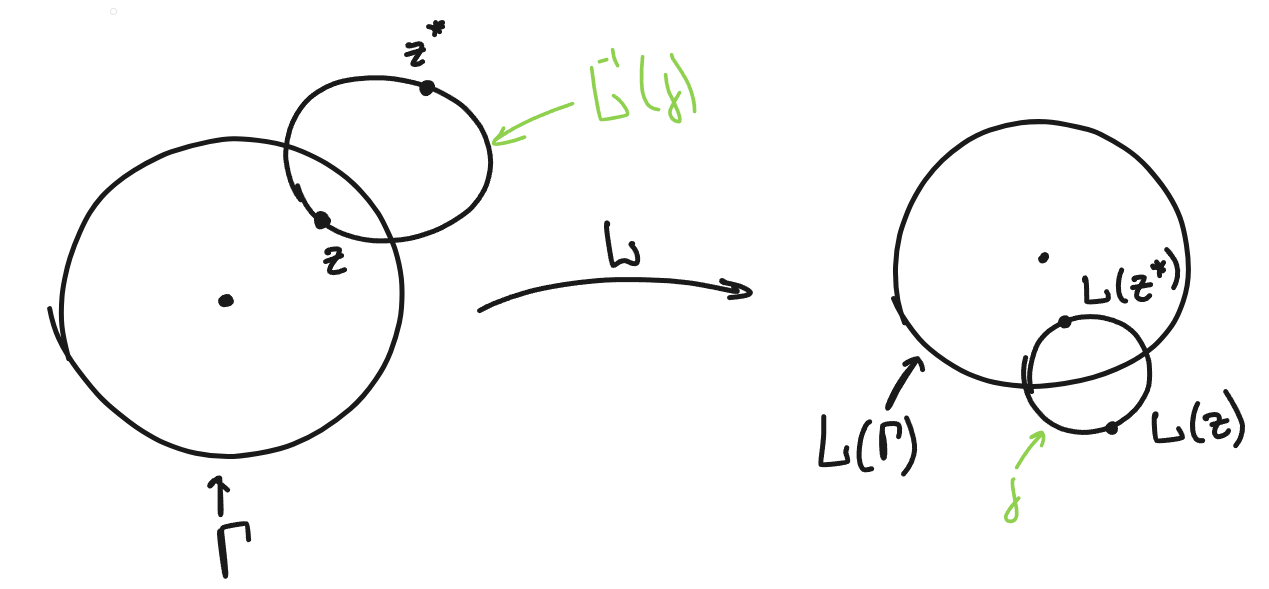
\includegraphics[scale=0.4]{answers/img/ans8.png}
    \label{pic08}
    \end{center}
\end{figure}

\begin{proof}
    \ \\
    Пусть $\gamma$ --- произвольная обобщенная окружность, проходящая через точки $L(z)$ и $L(z^*)$. Тогда $L^{-1}(\gamma)$ --- обобщенная окружность по круговому свойству ДЛО.\\[2mm]
    Так как $L(z)$, $L(z^*) \in \gamma$, то:\\
    $L^{-1}(L(z))=z \in L^{-1}(\gamma)$ и $L^{-1}(L(z^*))=z^*\in L^{-1}(\gamma)$.\\[2mm]
    По определению симметричных точек окружности $\Gamma$ и $L^{-1}(\gamma)$ ортогональны. ДЛО $L$ сохраняет углы, а значит $L(\Gamma)$ ортогональна $L(\gamma)$. 
\end{proof}

\newpage
\section{Стереографическая проекция. Расширенная комплексная плоскость и ее топология. Бесконечно удаленная точка, ее окрестности. Угол между кривыми в бесконечности. Дифференцируемость и конформность в бесконечности. Дробно-линейные функции как отображения расширенной комплексной плоскости.}



Выберем ДСК с осями $\xi,\eta,\zeta$, причем оси $\xi,\eta$ совпадают с осями $x,y$.
\begin{figure}[!ht]
    \begin{center}
    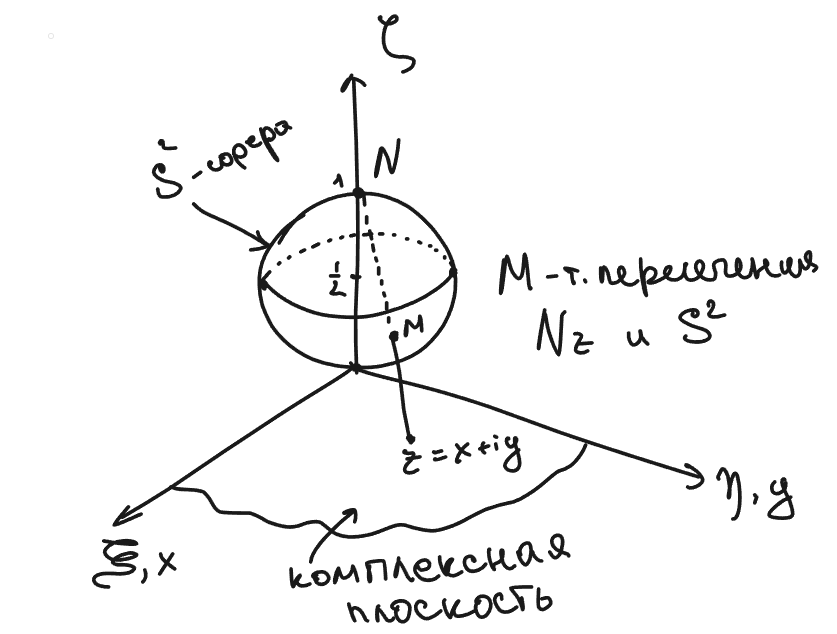
\includegraphics[scale=0.7]{answers/img/3.png}
    \label{pic04}
    \end{center}
\end{figure}
Рассмотрим сферу радиуса $\frac{1}{2}$ в этой системе координат, которая описывается уравнением 
$$
S^2: \xi^2 + \eta^2 + \left(\zeta - \frac{1}{2}\right)^2 = \left(\frac{1}{2}\right)^2
$$
а также луч, исходящий из точки $N(0,0,1)$, и пересекающий плоскость $0xy$ в точке (x,y), заданный параметрически:
$$
\begin{cases}
  \xi = 0 + tx \\
  \eta = 0 + ty \\
  \zeta = 1 + t \cdot (-1)
\end{cases}
$$

Точка пересечения луча со сферой $(\xi,\eta,\zeta)$ (подставляем в уравнение сферы уравнения луча):
\begin{gather*}
  t^2x^2 + t^2y^2 + \left(\frac{1}{2} - t\right)^2 = \left(\frac{1}{2}\right)^2 \\
  t^2(x^2 + y^2 + 1) - t = 0~~ | : t \neq 0 \\
  t = \frac{1}{1+x^2+y^2} = \frac{1}{1+|z|^2}
\end{gather*}
\begin{equation} \label{eq:forward}
\begin{cases}
  \xi = \frac{x}{1+x^2 + y^2} = \frac{x}{1+|z|^2} \\
  \eta = \frac{y}{1+x^2 + y^2} = \frac{y}{1+|z|^2} \\
  \zeta = \frac{x^2 + y^2}{1+x^2 + y^2} = \frac{|z|^2}{1+|z|^2}
\end{cases}
\end{equation}

Обратное отображение:
\begin{gather*}
\zeta = \frac{|z|^2 + 1 - 1}{1+|z|^2} \Rightarrow \frac{1}{1 + |z|^2} = 1 - \zeta \\
\Rightarrow \xi = x(1 - \zeta), \eta = y(1 - \zeta)
\Rightarrow 
\end{gather*}
\begin{equation}\label{eq:backwards}
\begin{cases}
  x = \frac{\xi}{1 - \zeta} \\
  y = \frac{\eta}{1 - \zeta}
\end{cases}
\end{equation}

Отображения (\ref{eq:forward}) и (\ref{eq:backwards}) являются однозначными отображениями между $\mathbb{C}$ и $S^2 \setminus N$, так как в преобразованиях не возникали неоднозначности.

$\overline{\mathbb{C}} = \mathbb{C} \cup \{\infty\}$. $\overline{\mathbb{C}}$ называется \textbf{расширенной комплексной плоскостью}. 

\textbf{Топология} $\overline{\mathbb{C}}$:

Открытое множество на $S^2$ -- $U \cap S^2$, где $U$ -- открытое в $\mathbb{R}^3$.

Условимся, что точке $N(0,0,1)$ соответствует точка $\infty$ поля $\overline{\mathbb{C}}$, тем самым определяется биекция между $S^2$ и $\overline{\mathbb{C}}$, точка $\infty$ называется \textbf{бесконечно удаленной точкой}.

\textbf{Окрестностью} $U$ бесконечно удаленной точки называется множество точек $z$, удовлетворяющих неравенству
$$
|z - z_0| > R, R\in \mathbb{R}
$$

Функция $f: U \rightarrow \overline{\mathbb{C}}$, $\infty\in U$, \textbf{дифференцируема в точке $\infty$}, если функция $\varphi(z) = f\left(\frac{1}{z}\right)$ дифференцируема в нуле.

Функция $f: U \rightarrow \overline{\mathbb{C}}$, $\infty\in U$, \textbf{конформна в точке $\infty$}, если функция $\varphi(z) = f\left(\frac{1}{z}\right)$ конформна в нуле.

\newpage
\section{Интеграл от функции комплексного переменного вдоль пути в $\mathbb{C}$. Его свойства.}


\textbf{Путь} -- параметризованная кривая, возможно с самопересечением (непрерывное отображение $\gamma$ : $[a, b]\subset \mathbb{R} \rightarrow \mathbb{C}$).\\[2mm]
Пусть $\gamma$ -- гладкий путь, то есть $\gamma$ : $z = z(t)$, $t \in J = [\alpha, \beta] \subset \mathbb{R}$, $z(t) \in \mathbb{C}$, $z(J) \subset \mathbb{C}$, функция $f(z)$ определена на $z(J)$ и функция \\ 
$f(z(t))$ : $J \rightarrow \mathbb{C}$ непрерывна (говорят, что $f$ непрерывна на $\gamma$).\\
Число \(\int_{\alpha}^{\beta} f(z(t))z'(t) \,dt\) называют \textbf{интегралом от функции $f$ вдоль пути $\gamma$} и обозначают \(\int_{\gamma} f(z) \, dz\), где $z(t) = x(t) + iy(t)$, $z'(t) = x'(t) + iy'(t)$.\\[2mm]
\textbf{Свойства интеграла:}
\begin{enumerate}
    \item Линейность: \(\int_{\gamma} [af(z) + bf(z)]\, dz\) $=$ $a$\(\int_{\gamma} f(z)\, dz\) $+$ $b$\(\int_{\gamma} f(z)\, dz\);
    \item Ориентированность:
    \begin{figure}[!ht]
    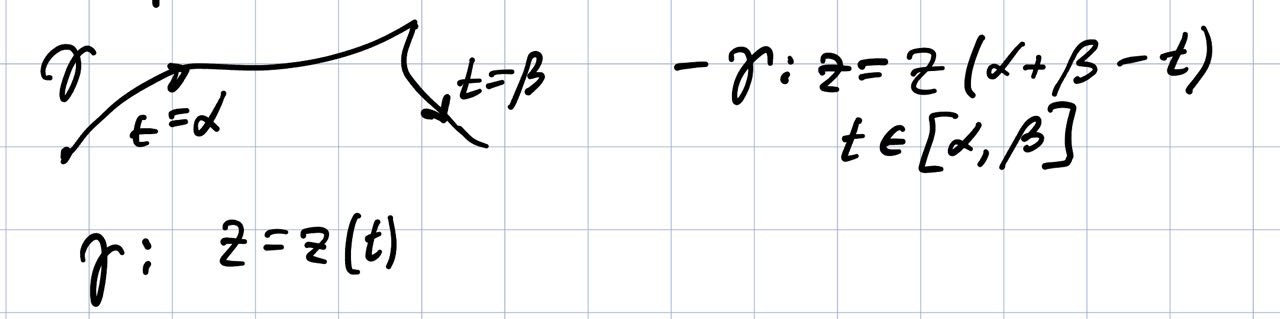
\includegraphics[scale=0.2]{answers/img/pic1.jpg}
    \end{figure}\\
    \(\int_{-\gamma} f(z)\, dz\) $=$ $-$\(\int_{\gamma} f(z)\, dz\);
    \item Аддитивность:\\
    \begin{figure}[!ht]
    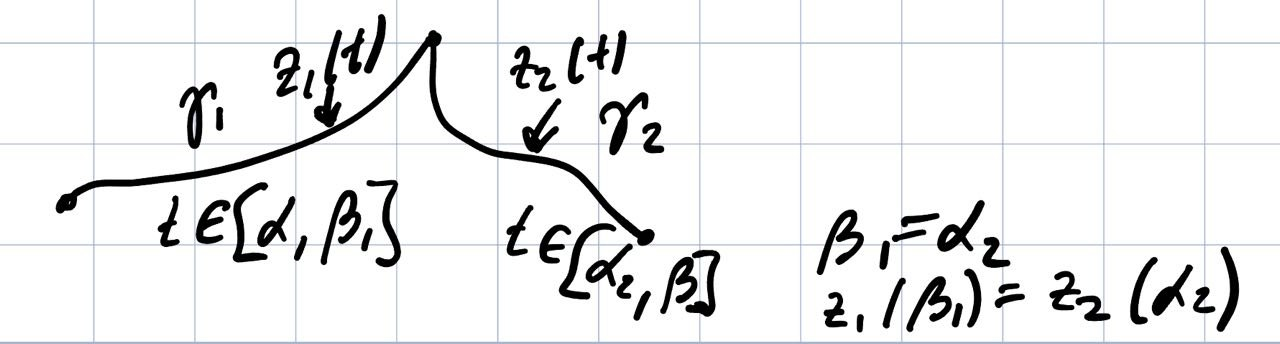
\includegraphics[scale=0.2]{answers/img/pic2.jpg}
    \end{figure}\\
    $\gamma_1 \cup \gamma_2$ : $z = 
    \begin{cases}
        z_1(t), t \in [\alpha, \beta_1];\\
        z_2(t), t \in [\alpha_2, \beta].
    \end{cases}$\\
    \(\int_{\gamma_1 \cup \gamma_2} f\, dz\) $=$ \(\int_{\gamma_1} f\, dz\) $+$ \(\int_{\gamma_2} f\, dz\);
    \item Независимость интеграла от выбора параметризации кривой:\\
    Пусть $\gamma$ : $z = z(t)$, $t \in [\alpha, \beta]$, $\gamma_1$ : $z = z_1(\tau)$ , $\tau \in [\alpha_1, \beta_1]$ -- два непрерывно дифференцируемых пути, $z_1(\tau) = z(t(\tau))$ $\forall \tau \in [\alpha_1, \beta_1]$, где $t = t(\tau)$ : $[\alpha_1, \beta_1] \rightarrow [\alpha, \beta]$ -- непрерывно дифференцируемая возрастающая функция, $f$ непрерывна на $\gamma$.\\
    Тогда \(\int_{\gamma} f\, dz\) $=$ \(\int_{\gamma_1} f\, dz\);
    \item Оценка интеграла:\\
    Если $f$ -- непрерывная функция на кусочно-гладком пути $\gamma$ : $z = z(t)$, $t \in [\alpha, \beta]$, то 
    |\(\int_{\gamma} f\, dz\)| $\leq$ \(\int_{\gamma} |f(z)||z'(t)|\, dt\)\\ 
    ( $|z'(t)|dt = |dz|$ -- дифференциал длины дуги).
\end{enumerate}

\begin{proof}
    \ \\
    4. Независимость интеграла:\\
    $\int\limits_{\gamma}  fdz = \int\limits_{\alpha}^{\beta} f(z(t))z'(t)dt =$\[
    \left | 
    t=t(\tau), \ 
    dt=t'(\tau)d\tau, \ 
    \frac{dz(t(\tau))}{d\tau} = \frac{dt}{d\tau}\frac{dz(t(\tau))}{dt}
    \right |    
    \]
    $ = \int\limits_{\alpha_1}^{\beta_1} f(z(t(z))) \cdot z'(t(\tau))t'(\tau)d\tau = \int\limits_{\alpha_1}^{\beta_1} f(z_1(\tau))z'(\tau)d\tau = \int\limits_{\gamma_1}dz$\\
    5. Оценка интеграла:\\
    Пусть $I=\int\limits_{\gamma} fdz \in \mathbb{C} = |I|\cdot \exp^{i\theta}$\\
    $|I|=\exp^{-i\theta}\cdot I = \int\exp^{-i\theta}f[z(t)]z'(t)dt$\\
    Обозначим $g(t) = \exp^{-i\theta}f[z(t)]z'(t)$.\\
    Тогда $|I| = \int\limits_{\alpha}^{\beta} Re \, g(t)dt+i\int\limits_{\alpha}^{\beta} Im \,g(t)dt\leq \int\limits_{\alpha}^{\beta}|g(t)|dt=\int\limits_{\alpha}^{\beta}|\exp^{-i\theta}|\cdot |f(z(t))|\cdot |z'(t)|dt$
\end{proof}

\newpage
\section{Теорема Коши для односвязных и многосвязных областей}
\textbf{Теорема 1 (Коши для односвязной области)}\\
Если $D \subset \mathbb{C}$ -- односвязная область, $f \in H(D)$ ($f$ голоморфна), $\gamma \subset D$ -- замкнутая кривая, то \(\int \limits_{\gamma} f\, dz\) $= 0$.


\begin{proof}
    \ \\
    Для случая, когда $f'(z)$ непрерывная в $D$:\\
    $z=x+iy$; $f(z)=u(x,y)+iv(x,y)$\\
    $I = \int\limits_{\gamma}fdz = \int\limits_{\alpha}^{\beta}f(z(t))z'(t)dt = \int \limits_{\alpha}^{\beta}[u(zx(t),y(t))+iv(x(t), y(t))]\cdot [x'(t)+it'(t)]dt = \int\limits_{\alpha}^{\beta}[u\cdot x'-v\cdot y')+i(uy'+vx')]dt=\int\limits_{\alpha}^{\beta}(ux'-vy')dt+i\int\limits_{\alpha}^{\beta}(uy'+vx')dt = \int\limits_{\gamma}udx-vdy +i\int\limits_{\gamma}udy+vdx=$
    Разрежем $\gamma$ на простые контуры $\gamma_i$:\\
    $\gamma=\bigcup\limits_{j=1}^{k}\gamma_j$, $G_j$ -- область внутри $\gamma_j$\\
    $I = \sum_{j=1}^k \left[ \oint\limits_{\gamma_j}u\,dx-v\,dy+i\oint\limits_{\gamma_j}v\,dx+u\,dy \right] =$\\
    $= \sum_j \left[ \iint\limits_{G_j}\left(-\frac{\partial v}{\partial x}-\frac{\partial u}{\partial y} \right)dx\,dy + i\iint\limits_{G_j}\left(\frac{\partial u}{\partial x}-\frac{\partial v}{\partial y} \right)dx\,dy \right] = 0$
\end{proof}


\textbf{Теорема 2 (Коши для многосвязной области)}\\
\begin{figure}[!ht]
\begin{center}
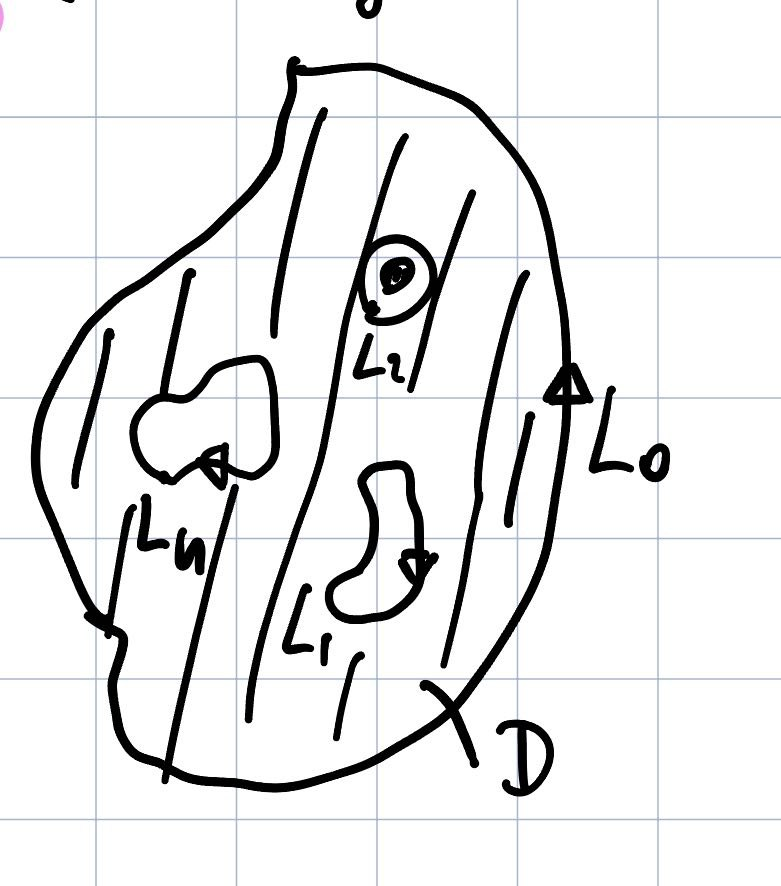
\includegraphics[scale=0.2]{answers/img/pic3.jpg}
\end{center}
\end{figure}\\
Пусть многосвязная область $D$ ограничена внешним контуром $L_0$ и внутренними контурами $L_1$, ..., $L_n$, контуры $L_1$, ..., $L_n$ -- кусочно-гладкие, $f \in H(D \cup L_0 \cup L_1 \cup$ ... $\cup L_n)$.\\
Тогда \(\int_L f\, dz\) $= 0$, где $L = L_0 \cup L_1 \cup$ ... $\cup L_n$, обход $L_0$ -- против часовой стрелки, $L_1$, ..., $L_n$ -- по часовой стрелке.\\
\textbf{Замечание.} \(\oint_{L_0} f\, dz\) 
$= \sum_{i = 1}^{n}$\(\oint_{L_i} f\, dz\), где обход $L_0$, $L_1$, ..., $L_n$ против часовой стрелки.


\begin{proof}
    \ \\
    С помощью разрезов $\gamma_1, ..., \gamma_n$ получим односвязную область $D^*$. Тогда $D=D^*\cup\gamma_1\cup...\cup\gamma_n$.\\
    Так как $D^*$--односвязная, то $0=\int\limits_{D^*}fdz = $\\
    Граница $D^* = L_0\cup\gamma_1\cup-\gamma_1\cup L_1 \cup...\cup\gamma_n\cup-\gamma_n\cup L_n$.\\
    Тогда из аддитивности и ориентированности:\\
    $=\int\limits_{L_0}fdz+\sum_{i=1}^n\left[ \int\limits_{\gamma_i}fdz+\int\limits_{-\gamma_i}fdz+\int\limits_{L_i}fdz \right] = \int\limits_{L}fdz=0$
\end{proof}

\newpage
\section{Интегральная формула Коши для функции и ее производных.}


\textbf{Интегральная формула Коши для голоморфных функций:}

Пусть $D$ --- односвязная область в $\mathbb{C}$, $\partial D$ --- граница $D$, $f\in H(D\cup \partial D).$

Тогда для $z_0 \in D$:
$$f(z_0)=\frac{1}{2\pi i} \cdot \oint\limits_{\partial D} \frac{f(z)}{z-z_0}dz$$

\begin{proof}
    \ \\
    \begin{figure}[!ht]
        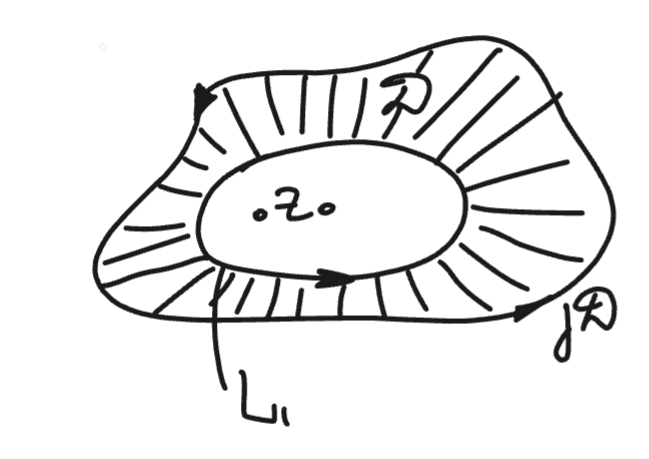
\includegraphics[scale=0.6]{answers/img/ans9.png}
    \end{figure}\\
    1) Пусть $L_1$ -- простой контур, $L_1 \subset D$\\
    Пусть $D_1$ -- область внутри $L_1$, $G=D\backslash D_1\backslash L_1$ -- многосвязная область\\
    По т. Коши для многосвязной области:
    $$\int\limits_{\partial G}\frac{f(z)}{z-z_0}dz=0,$$
    т.к. $\frac{f(z)}{z-z_0} \in H(G)$\\
    Имеем $\partial G = \partial D \cup (-L_1)$:\\
    $$\oint\limits{\partial D}\frac{f(z)}{z-z_0}dz-\oint\limits_{L}\frac{f(z)}{z-z_0}dz=0$$

    2) Пусть $\gamma: \, z=z+r\cdot e^{it}, \ t\in[0, 2\pi], \ r>0$\\
    $f(z)=(z-a)^n; \ n\in \mathbb{Z}$\\
    $\int\limits_{\gamma}(z-a)^n dz = \int\limits_0^{2\pi} (a+r\cdot e^{it}-a)^n\cdot r\cdot ie^{it}dt = r^{n+1}\cdot i \cdot \int\limits_0^{2\pi} e^{it(n+1)}dt \Rightarrow$\\
    $\Rightarrow \oint\limits_{L_1}\frac{dz}{z-z_0} = 2\pi i,$
    где $L_1$ -- окр-ть с центром в точке $z_0$\\

    3) Пусть $\sigma_1$ -- радиус $L_1$ и $L_1 \subset D$\\
    $I = \left| \frac{1}{2\pi i } \oint\limits_{L_1} \frac{f(z)}{z-z_0}dz-f(z_0) \right| = \left| \frac{1}{2\pi i} \oint\limits_{L_1} \frac{f)(z)}{z-z_0}dz - f(z_0)\frac{1}{2\pi i}\int\limits_{L_1} \frac{dz}{z-z_0}\right| = $\\
    $= \left| \frac{1}{2\pi i}\oint\limits_{L_1} \frac{f(z)-f(z_0)}{z-z_0}dz \right| \leq \frac{1}{2\pi |i|} \oint\limits_{L_1}\left| \frac{f(z)-f(z_0)}{z-z_0} \right|z'(t)dt$\\

    4) Так как $f \in H(D)$, то $\forall \varepsilon > 0 \, \exists \delta (\varepsilon)>0: \, |z-z_0|<\delta \rightarrow |f(z)-f(z_0)|<\varepsilon$\\
    Имеем $z\in L_1: \ |z-z_0| = \sigma_1$:\\
    $\left| \frac{f(z)-f(z_0)}{z-z_0} \right|< \frac{\varepsilon}{\sigma_1}: \ \oint\limits_{L_1}|z'(t)|dt$ -- длина $L_1$, то есть $2\pi \sigma_1$\\
    Тогда $I \leq \frac{1}{2\pi}\cdot \frac{\varepsilon}{\gamma_1}\cdot 2\pi \sigma_1 = \varepsilon \Rightarrow$ не зависит от $\varepsilon$ 

\end{proof}
\textbf{Интегральная формула Коши для производных:}

Пусть $f\in H(D): \ G\cup \partial G \subset D; \ D$ --- область, ограниченная конечным числом замкнутых кривых, $z_0 \in G$

Тогда:
$$f^{(n)}(z_0) = \frac{n!}{2\pi i} \int\limits_{\partial G}\frac{f(\xi)}{(\xi-z_0)^{n+1}}d\xi$$

\begin{proof}
    \ \\
    По теоремам о разложении голоморфной функции в степенной ряд и теореме о единственности разложения в степенной ряд:\\
    $c_n=\frac{1}{2\pi} \oint\limits_{\gamma r} \frac{f(\xi)d\xi}{(\xi-z_0)^{n+1}}$; $\oint\limits_{\gamma r}...=\oint\limits_{\gamma G}$
\end{proof}
\newpage
\section{Степенные ряды в $\mathbb{C}$, их свойства. Голоморфность суммы степенного ряда.}

Ряд $\sum_{n=0}^\infty c_n(z-z_0)^n$ --- \textbf{степенной} ряд, $c_n \in \mathbb{C}$.\\[2mm]

\textbf{Свойства:}
\begin{enumerate}
    \item Теорема Абеля:\\
    Если степенной ряд $\sum_{n=0}^\infty c_n(z-z_0)^n$ сходится в точке $z_1$, то этот ряд сходится в круге $U=\{z\in \mathbb{C}: \, |z-z_0|<|z_1-z_0|\}$ и на любм компакте $K \subset U$ он сходится равномерно.
    \item Теорема Коши-Адамара:\\
    Пусть для ряда $A: \ \sum_{n=0}^\infty c_n(z-z_0)^n$ имеем $\overline{\lim\limits_{n\to\infty}\limits}\sqrt[n]{|c_n|} = \frac{1}{R}$, где $,\leq R \leq \infty$.\\
    Тогда в любой точке $z: \ |z-z_0|<R$ ряд сходится и в любой точке $z: \ |z-z_0|>R$ ряд расходится.
\end{enumerate}

\textbf{Голоморфность суммы степенного ряда:}\\[2mm]
Пусть в круге $U=\{z\in \mathbb{C}: \, |z-z_0|<R\}$  $S(z) = \sum_{n=0}^\infty c_n (z-z_0)^n$.\\
Тогда $S \in H(U_R(z_0))$ и $S'(z)=\sum_{n=1}^\infty n\cdot c_n(z-z_0)^{n-1} \ (*)$

\begin{proof}
    \ \\
    $r: \ 0<r<R$ -- произвольные.\\
    Пусть $z_1 \in U_R(z_0): \ |z-z_0| > r$\\
    $\forall z \in U_r(z_0) = \{z: |z-z_0|<r\}:$\\
    $|n\cdot C_n(z-z_0)^{n-1}| = n\left|C_n\frac{(z-z_0)^{n-1}}{(z_1-z_0)^n}\right|\cdot |(z_1-z_0)^n|=n\frac{1}{|z_1-z_0|}\cdot |C_n (z_1-z_0)^n|\cdot \left|\frac{z-z_0}{z_1-z_0}\right|^{n-1}\leq n\frac{M}{|z_1-z_0|}\rho^{n-1}$,\\
    где $M > |C_n (z_1-z_0)^n|, \ \rho = \left|\frac{z-z_0}{z_1-z_0}\right|$\\
    То есть ряд $\sum_{n=1}^\infty n\frac{M}{|z_1-z_0|}\rho^{n-1}=\frac{M}{|z_1-z_0|}\sum_{n=1}^\infty n\rho^{n-1}$ -- мажорирующий для ряда $(*)$.\\
    Ряд $\sum_{n=1}^\infty n\rho^{n-1}$ сходится при $\rho \in (0; 1)$ как ряд из производных ряда $\sum_{n=1}^\infty\rho^n$. Тогда по признаку Вейерштрасса ряд $(*)$ сходится равномерно и абсолютно в $U_r(z_0)$.

    Для любой замкнутой кривой $\gamma \subset U_r(z_0)$ по теореме Коши:\\
    $\oint\limits_{\gamma}\left( \sum_{n=1}^\infty n C_n (z-z_0)^{n-1} \right)dz=\sum_{n=1}^\infty C_n \oint\limits_{\gamma}(z-z_0)^{n-1}dz=0$\\
    Значит функция $g(z)=\sum_{n=1}^\infty n\cdot C_n(z-z_0)^{n-1}$ имеет первообразную в $U_r(z_0)$, которая равна:\\
    $\int\limits_{z_0}^z g(\xi)d\xi = \int\limits_{z_0}^z\sum_{n=1}^{\infty} n\cdot C_n (\xi-z_0)^{n-1}d\xi=\sum_{n=1}^{\infty} n C_n \frac{(z-z_0)^n}{n} = S(z)-S(z_0) = S(z)-C_0$.\\
    Следовательно $S \in H(U_r(z_0)) \forall r \in (0; R)$.\\
    Поэтому $S \in H(U_R(z_0))$ и $S'=g$.
\end{proof}

\textbf{Следствия} из этой теоремы:
\begin{enumerate}
    \item Производная функции $f\in H(d)$ голоморфна в $D$
    \item Если функция $f$ в области $D$ первообразную, то $f \in H(D)$
    \item $f \in H(D) \Rightarrow f$ бесконечно дифференцируема и все ее производные голоморфны
\end{enumerate}

\section{Теорема о разложении голоморфной функции в ряд Тейлора. Неравенства Коши для коэффициентов ряда Тейлора. Теорема Лиувилля.}

\textbf{Теорема о разложение голоморфной функции в ряд Тейлора:}\\[2mm]
Пусть $D$ -- область в $\mathbb{C} \ f \in H(D), \ z_0 \in D, U_R(z_0) = \{z \in \mathbb{C}: |z-z_0| < R\} \subset D$. \\[2mm]
Тогда $f(z) = \sum_{n=0}^{\infty}c_n \cdot (z-z_0)^n, \ z \in U_R(z_0), \ c_n = \frac{1}{2\pi i} \int \limits_{{\gamma}_r} \frac{f(\xi)}{(\xi-z)^{n+1}} d\xi, \ \gamma_r = \{z \in \mathbb{C}: |z-z_0| = r\}$


\begin{proof}
	\ \\
	По интегральной формуле Коши: \\[2mm]
	$f(z) = \frac{1}{2 \pi i} \int \limits_{{\gamma}_r} \frac{f(\xi)}{\xi - z} d\xi$ если $|z-z_0| < r$\\[2mm]
	$\frac{1}{\xi - z} = \frac{1}{\xi - z_0 - (z - z_0)} = \frac{1}{\xi - z_0} \cdot \frac{1}{1 - \frac{z-z_0}{\xi - z_0}} \ (=)$\\[2mm]
	$\frac{|z-z_0|}{|\xi - z_0|} = \frac{|z - z_0|}{r} < 1$\\[2mm]
	$(=) \ \frac{1}{z-z_0} \cdot \sum_{n=0}^{\infty} \left( \frac {z-z_0}{\xi - z_0}\right)^n, \ \frac{1}{2 \pi i}f(z)$ -- непрерывна. \\[2mm]
	Тогда $ \ \frac{1}{2 \pi i}f(z) \cdot \frac{1}{\xi - z} = \frac{1}{2 \pi i} \sum \frac{f(\xi)(z-z_0)^n}{0}$ -- сходится равномерно, значит можно интегрировать почленно. \\[2mm]
	Тогда получаем утверждение теоремы:
	$$
	f(z) = \frac{1}{2 \pi i} \int \limits_{{\gamma}_r} \sum_{n=0}^{\infty}\frac{f(\xi) (z - z_0)^n}{(\xi - z_0)^{n+1}}d\xi = \frac{1}{2 \pi i}\sum_{n=0}^{\infty}(z-z_0)^n \int \limits_{{\gamma}_r} \frac{f(\xi)}{(z-z_0)^{n+1}}
	$$
\end{proof}


\textbf{Неравенство Коши для коэффициентов ряда Тейлора:}\\[2mm]
Пусть функция $f \in H(\overline{U})$, где $U = \{ z: |z-z_0|d \leq r\}$ и $\partial\overline{U} = {\gamma}_r, \ |f(z) \leq M$. \\[2mm]
Тогда коэффициенты ряда Тейлора $f$ удовлетворяют следующему неравеству: $|c_n| \leq \frac{M}{r^n}$ 


\begin{proof}
	\ \\
	\begin{equation*}
		|c_n| = |\frac{1}{2 \pi i} \int \limits_{{\gamma}_r} \frac{f(\xi)}{(\xi - z_0)^{n+1}}d\xi| \leq \frac{1}{2 \pi} \cdot \frac{M}{r^{n+1}} \cdot 2 \pi r = \frac{M}{r^n},
	\end{equation*}
	так как $|f(\xi)| \leq M$ и $(\xi - z)^{n+1} \leq r^{n+1}$
\end{proof}


\textbf{Теорема Лиувилля:}\\[2mm]
$f \in H(\mathbb{C})$ и $f$ -- ограниченная функция $\Rightarrow \ f = const$ 


\begin{proof}
	По теореме о разложении голоморфной функции в ряд Тейлора 
	функция $f$ представима в виде $f = \sum_{n=0}^{\infty} c_n (z - z_0)^n$ внутри окружности любого радиуса $R$,
	причем по этой же теореме коэффициенты ряда не зависят от $R$.\\[2mm]
	Тогда из неравенства Коши для коэффициентов ряда Тейлора:
	$$
	|c_n| \leq \frac{M}{R^n}
	$$
	Из того что $R$ произвольный следует, что $c_n = 0$ для
	любого $n$, а значит $f = const$
\end{proof}


\newpage
\section{Бесконечная дифференцируемость голоморфных функций. Единственность разложения в степенной ряд. Теорема Морера. Эквивалентность голоморфности в смысле Римана, Коши и Вейерштрасса.}


\textbf{Голоморфность суммы степенного ряда:}\\[2mm]
Пусть в круге $U=\{z\in \mathbb{C}: \, |z-z_0|<R\}$  $S(z) = \sum_{n=0}^\infty c_n (z-z_0)^n$.\\
Тогда $S \in H(U_R(z_0))$ и $S'(z)=\sum_{n=1}^\infty n\cdot c_n(z-z_0)^{n-1} \ (*)$

\begin{proof}
    \ \\
    $r: \ 0<r<R$ -- произвольные.\\
    Пусть $z_1 \in U_R(z_0): \ |z-z_0| > r$\\
    $\forall z \in U_r(z_0) = \{z: |z-z_0|<r\}:$\\
    $|n\cdot C_n(z-z_0)^{n-1}| = n\left|C_n\frac{(z-z_0)^{n-1}}{(z_1-z_0)^n}\right|\cdot |(z_1-z_0)^n|=n\frac{1}{|z_1-z_0|}\cdot |C_n (z_1-z_0)^n|\cdot \left|\frac{z-z_0}{z_1-z_0}\right|^{n-1}\leq n\frac{M}{|z_1-z_0|}\rho^{n-1}$,\\
    где $M > |C_n (z_1-z_0)^n|, \ \rho = \left|\frac{z-z_0}{z_1-z_0}\right|$\\
    То есть ряд $\sum_{n=1}^\infty n\frac{M}{|z_1-z_0|}\rho^{n-1}=\frac{M}{|z_1-z_0|}\sum_{n=1}^\infty n\rho^{n-1}$ -- мажорирующий для ряда $(*)$.\\
    Ряд $\sum_{n=1}^\infty n\rho^{n-1}$ сходится при $\rho \in (0; 1)$ как ряд из производных ряда $\sum_{n=1}^\infty\rho^n$. Тогда по признаку Вейерштрасса ряд $(*)$ сходится равномерно и абсолютно в $U_r(z_0)$.

    Для любой замкнутой кривой $\gamma \subset U_r(z_0)$ по теореме Коши:\\
    $\oint\limits_{\gamma}\left( \sum_{n=1}^\infty n C_n (z-z_0)^{n-1} \right)dz=\sum_{n=1}^\infty C_n \oint\limits_{\gamma}(z-z_0)^{n-1}dz=0$\\
    Значит функция $g(z)=\sum_{n=1}^\infty n\cdot C_n(z-z_0)^{n-1}$ имеет первообразную в $U_r(z_0)$, которая равна:\\
    $\int\limits_{z_0}^z g(\xi)d\xi = \int\limits_{z_0}^z\sum_{n=1}^{\infty} n\cdot C_n (\xi-z_0)^{n-1}d\xi=\sum_{n=1}^{\infty} n C_n \frac{(z-z_0)^n}{n} = S(z)-S(z_0) = S(z)-C_0$.\\
    Следовательно $S \in H(U_r(z_0)) \forall r \in (0; R)$.\\
    Поэтому $S \in H(U_R(z_0))$ и $S'=g$.
\end{proof}

\textbf{Следствие} из этой теоремы:
Производная функции $f\in H(D)$ голоморфна в $D$
\begin{proof}
    \ \\
    $z_0 \in D$ -- произвольная точка множества $D \ \Rightarrow$ $z_0$ -- внутренняя точка $D$, 
    так как $D$ -- открытое множество $\Rightarrow$ \\[2mm]
    $\exists R > 0: U_R(z_0) \subset D \Rightarrow$ \\[2mm]
    $(\text{теорема о разложении голоморфной функции в ряд})$ \\[2mm] 
    $f(z) = \sum_{n=0}^{\infty}c_n (z - z_0)^n \Rightarrow$ (голом. степенного ряда)\\[2mm]
    $\Rightarrow \ f'(z)$ -- сумма степенного ряда, значит голоморфна 
\end{proof}

Из следствия 1 теоремы о разложении функции в степенной 
ряд следует бесконечная дифференцируемость голоморфных функций.


\textbf{Теорема о единственности разложения в степенной ряд:}\\[2mm]
Если в $U_R(z_0) \ f(z) = \sum_{n=0}^{\infty}c_n (z-z_0)^n$, то $c_n = \frac{f^{(n)}(z_0)}{n!}$


\begin{proof}
	\ \\
	\begin{equation*}
	\begin{gathered}
		f(z_0) = c_0 \\
		f'(z_0) = \sum_{n=1}^{\infty}nc_n(z-z_0)^{n-1} = c_1 \\
		\dots \\
		f^{(k)} = \sum_{n=k}^{\infty} n(n-1)\ldots(n-k+1)c_n(z-z_0)^{n-k} = \\ 
		= k(k-1) \cdot \ldots \cdot 1 = k!c_k \Rightarrow \\ 
		\Rightarrow c_k = \frac{f^{(k)}(z_0)}{k!}
	\end{gathered}
	\end{equation*}
\end{proof}


\textbf{Теорема Морера:}\\[2mm]
Пусть $D \subset \mathbb{C}$ -- область, $f \in C(D)$ и $\int \limits_{\partial \Delta}f(\xi)d\xi = 0$
для произвольного треугольника $\Delta$ при $\Delta \cup \partial \Delta \subset D$. \\[2mm]
Тогда $f \in H(D)$


\begin{proof}
	\ \\
	Пусть $a \in D$ -- призвольная точка. \\[2mm]
	Так как $D$ -- открытое, то $\exists r: U_r(a) \subset D$ \\[2mm]
	Рассмотрим функцию $F = \int \limits_{[a, z]} f(\xi)d\xi$, $z \in U_r(z_0)$ \\[2mm]
	Аналогично доказательству теоремы о первообразной $F \in H(D)$ и $F'(z) = f(z)$ \\[2mm]
	Из голоморфности производной голоморфной функции следует утверждение теоремы
\end{proof}


\textbf{Теорема об эквивалетности трех определений голоморфности:}
3 следующих утверждения эквивалентны:\\[2mm]
R) функция $f$ в некоторой окрестности $U(a)$ имеет комплексную производную (Риман) \\[2mm]
C) $f \in C(U(a))$ и $\int \limits_{\partial \Delta}f(z)dz = 0$ для любого треугольника $\Delta \subset U(a)$ (Коши)\\[2mm] 
W) функция $f$ разложима в степенной ряд в окрестности точки $a$ по $(z-a)$ (Вейерштрасс)


\begin{proof}
	\ \\
	$R) \Rightarrow C)$ -- из теоремы Коши \\[2mm]
	$R) \Rightarrow W)$ -- по теореме о разложении голоморфной функции степенной ряд \\[2mm]
	$W) \Rightarrow R)$ -- теорема о голоморфности суммы степенного ряда \\[2mm]
	$C) \Rightarrow R)$ -- по теореме Морера
\end{proof}

\newpage
\section{Нули голоморфной функции, их свойства. Теорема единственности. Вычисление порядка нуля.}

\textbf{Определение:}\\[2mm]
Нулем функции $f$ называется точка $a \in \mathbb{C}: f(a) = 0$


\textbf{Теорема:}\\[2mm]
Если $f(a) = 0, \ f$ голофорфна в точке $a$, и $f \equiv 0$ в какой то окрестности точки $a$,
то $\exists n \in \mathbb{N}: f(z) = (z - a)^n\varphi(z)$, где $\varphi(z) \neq 0$ и $\varphi$ голоморфна в точке $a$


\begin{proof}
    \ \\
    По теореме о разложении голоморфной функции в степенной ряд:\\[2mm]
    $f(z) = \sum_{n=0}^{\infty} c_n (z-a)^n$ в некоторой окрестности точки $a$\\[2mm]
    $f(a) = c_0 = 0, \ \exists n \in \mathbb{N} \ c_n \neq 0$ (иначе $f(z) \equiv 0$)\\[2mm]
    Пусть $n \in \mathbb{N}$ -- такое, что $c_0 = c_1 = \ldots = c_{n-1} = 0$. Тогда \\[2mm]
    $f(z) = \sum_{n=0}^{\infty}c_n (z-a)^n = \sum_{k=n}^{\infty}c_k(z-a)^k = (z-a)^n\sum_{k=n}^{\infty}c_k(z-a)^{k-n}$\\[2mm]
    Функция $\varphi(z) = \sum_{n=k}^{\infty}c_k(z-a)^{k-n}$ и есть искомая функция (голоморфна и не ноль в $a$)
\end{proof}


\textbf{Следствие:}\\[2mm]
Если $f(a) = 0$, $f$ голоморфна в точке $a$, то
существует выколотая окрестность точки $a$, где функция не имеет нулей,
то есть ее нули -- изолированные точки


\textbf{Теорема о порядке нуля голомофрной функции:}\\[2mm]
Порядок нуля $a \in \mathbb{C}$ голоморфной функции $f$ 
совпадает с $n$ в формуле $f(z) = (z-a)^n\varphi(z)$


\begin{proof}
    \ \\
    В ходе доказательства теоремы o представлении
    голоморфной функции имеющей нуль было показано,\\[2mm] 
    что $c_0 = \ldots c_{n-1} = 0$. Из того что $c_k = f^{(k)}(a)$ 
    следует доказательство теоремы
\end{proof}


\textbf{Теорема единственности:}\\[2mm]
Если $D$ -- область в $\mathbb{C}$; $f_1, f_2 \in H(D), \ \forall z \in \mathcal{E} \subset D: f_1 = f_2$,\\[2mm]
$a$ -- предельная точка множества $\mathcal{E}$ и $a \in D$, то $f_1 = f_2$ на всем $D$


\begin{proof}
    \ \\
    $f = f_1 - f_2 \in H(D), \ \mathcal{R} = \{z \in D: f_1 = f_2\}$. \\[2mm] 
    Тогда $a$ -- предельная точка множества $\mathcal{R}$ \\[2mm]
    Тогда есть последовательность $\{z_n\}, \ z_n \rightarrow a$ при $n \rightarrow \infty$. \\[2mm]
    Из непрерывности $f$ следует что $\lim \limits_{z_n}f(z_n) = 0$, а \\[2mm]
    Из того что $a$ -- предельная точка множества $\mathcal{R}$ и следствия теоремы следует, что \\[2mm] 
    $f \equiv 0 \Rightarrow f_1 = f_2$ в некоторой окрестности точки $a$ \\[2mm]
    Из того что $a$ -- произвольная предельная точка имеем, что $\mathcal{R}$ -- замкнутное подмножество $D$ \\[2mm]
    Из связности $D$ следует, что $Int \mathcal{R} = D$
\end{proof}

\newpage
\section{Ряды Лорана, их области сходимости. Теоремы о разложении голоморфной функции и о единственности разложения в ряд Лорана. Неравенство Коши для коэффициентов ряда Лорана.}

Ряд Лорана:
$$
\sum\limits_{n=-\infty}^{+\infty} c_n(z-a)^n = \sum\limits_{n=-1}^{-\infty}c_n(z-a)^n + \sum\limits_{n=0}^{\infty}c_n(z-a)^n
$$

Первая сумма, с отрицательными коэффициентами,\\ $\sum\limits_{n=-1}^{-\infty}c_n(z-a)^n$, называется \textbf{главной частью}.

Вторая сумма называется \textbf{правильной частью}.

Ряд Лорана сходится, когда сходятся оба ряда.

Ясно, что правильная часть сходится, если  
$$|z - a| < R_1$$
где $R$ -- некоторое действительное число.
Аналогичным образом при замене $\xi = \frac{1}{z - a}$ главная часть преобразуется к обычному ряду
$$
\sum\limits_{n=-1}^{-\infty}c_n\xi^{-n}=\sum\limits_{k=1}^{\infty}c_{-k}\xi^{k}
$$
откуда $\xi<R_2$, где $R_2$ -- некоторое действительное число, откуда
$$|z - a| > R_2$$

Таким образом получаем два условия сходимости ряда Лорана, оба из которых должны выполняться для сходимости ряда, а значит областью сходимости ряда Лорана (за исключением граничных случаев) является кольцо:

\begin{center}
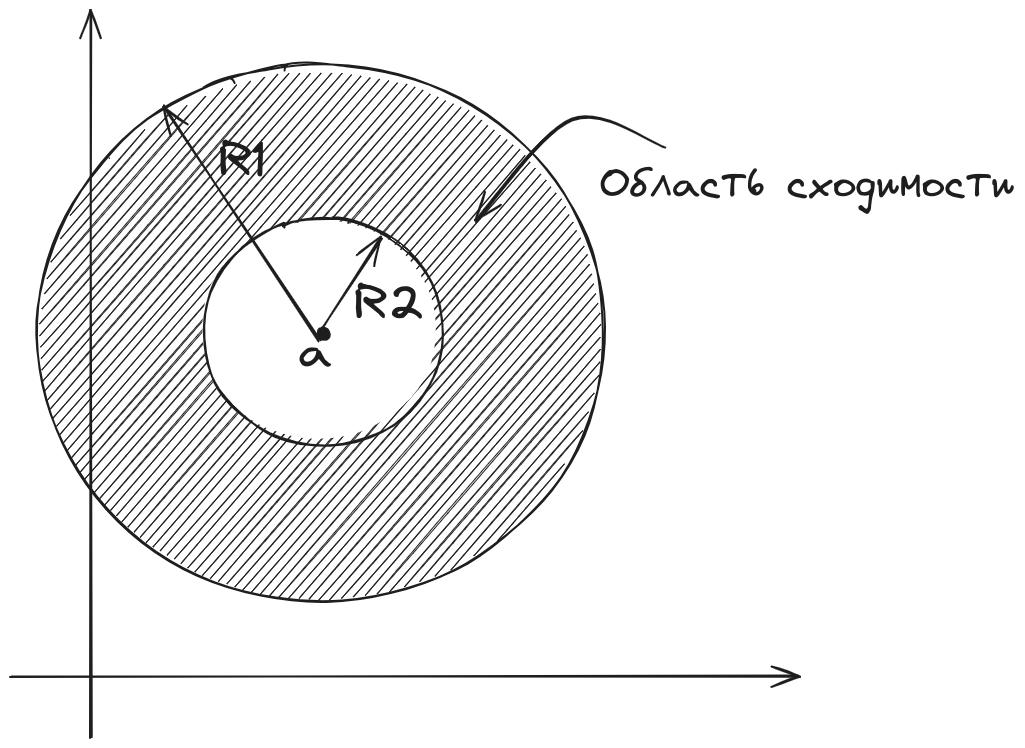
\includegraphics[scale=0.3]{answers/img/rng.png}
\end{center}

\textbf{Теорема Лорана}.\\[2mm]
Пусть $0\le R_2 < R_1 \le \infty$, $V = \{z\in\mathbb{C} ~~|~~ R_2 < |z - a| < R_1\}, f\in H(V)$.

Тогда $f(z) = \sum\limits_{-\infty}^{+\infty}c_n (z - a)^n$, где
$$
c_n = \frac{1}{2\pi i}\oint\limits_{|z - a| = \rho} \frac{f(\xi)}{(\xi - a)^{n + 1}} d\xi
$$
$n\in\mathbb{Z}, R_2 < \rho < R_1$

\begin{proof}
    \ \\
    
    \begin{figure}[h]
        \centering
        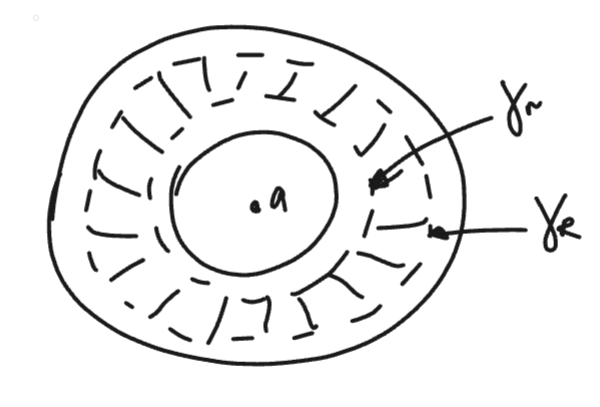
\includegraphics[width=0.4\linewidth]{answers/img/ans14.png}
    \end{figure}
    Пусть $r, R$ -- такие, что $R_2<r<R<R_1$.\\
    Тогда $V'=\{z\in \mathbb{C}: r<|z-a|<R\}$\\
    $\gamma V'=\gamma_r(a)\cup \gamma_R(a)\subset V, a\in V'$\\
    Интегральная формула Коши: $f(z)=\frac{1}{2\pi i}\cdot \int\limits_{\gamma V'}\frac{f(\xi)}{\xi-z}d\xi = \frac{1}{2\pi i}\oint\limits_{\gamma_R(a)}...-\frac{1}{2\pi i}\oint\limits_{\gamma_r(a)}... (=)$\\
    На $\gamma_R(a)$ обход против часовой стрелки:\\
    $\frac{1}{\xi-z}=\frac{1}{(\xi-a)(1-\frac{z-a}{\xi-a})}=\sum_{n=0}^\infty \frac{(z-a)^n}{(\xi-a)^{n+1}} = \frac{1}{(\xi-a)-(z-a)}=\frac{-1}{(z-a)(1-\frac{\xi-a}{z-a})}=-\frac{1}{z-a}\sum_{n=0}^\infty \frac{(\xi-a)^n}{(z-a)^n}=-\sum_{n=0}^\infty \frac{(\xi-a)^n}{(z-a)^{n+1}} = -\sum_{k=-1}^{-\infty} \frac{(z-a)^k}{(\xi-a)^{k+1}}$\\
    $(=) \sum_{n=0}^{+\infty} \frac{1}{2\pi i} \oint\limits{\gamma_R(a)\to\gamma_\rho(a)}f(\xi) \frac{(z-a)^n}{(\xi-a)^{n+1}}d\xi =$\\
    $=\sum_{k=-1}^{+\infty}\frac{1}{2\pi i}\cdot \oint\limits_{\gamma_r(a)\to \gamma_\rho(r)}f(\xi)\frac{(z-a)^k}{(\xi-a)^{k+1}}d\xi = \sum\limits_{n=0}^{+\infty} c_n(z-a)^n+$\\
    $+\sum_{k=-1}^{-\infty}c_k(z-a)^{-k}$ 
    
\end{proof}

\textbf{Теорема о единственности разложения в ряд Лорана.}\\[2mm]
Если в кольце $V = \{z\in\mathbb{C} ~~|~~ r < |z - a| < R\}$
$$
(*) f(z) = \sum\limits_{-\infty}^{+\infty}c_n(z - a)^n
$$
то
$$
c_n = \frac{1}{2\pi i}\oint\limits_{|z - a| = \rho} \frac{f(\xi)}{(\xi - a)^{n + 1}} d\xi
$$
где $n\in\mathbb{Z}, r < \rho < R$

\begin{proof}
    \ \\
    Ряд сходится равномерно на $\gamma$, т.к.:\\
    $f(z)=\sum_{n=0}^\infty c_n(z-a)^n + \sum_{k=1}^\infty c_{-k}(z-a)^{-k}$\\
    1.\\
    $|c_n(z-a)^n|=|c_n|\cdot|z-a|^n=|c_n|\rho^n < |c_n|R^n, z=a+\rho e^{it}$\\
    $r<r_1<\rho<R_1<R$\\
    $\sum|c_n|R^n$ -- сходится, значит по признаку Вейерштрасса первая часть  $f(z)$ сходится равномерно.\\
    2.\\
    $|c_{-k}(z-a)^{-k}|=\frac{|c_{-k}|}{|z-a|^k}=\frac{|c_{-k}|}{\rho^k}<\frac{|c_{-k}|}{r_1^k}$;\\
    $\sum \frac{|c_{-k}}{r_1^k}$ сходится, значит вторая часть сходится равномерно.\\[2mm]
    $f(z)\cdot (z-a)^{-k-1}=\sum_{n=-\infty}^\infty c_n(z-a)^{n-k-1}\Rightarrow \oint\limits_{\gamma}\frac{f(z)}{(z-a)^{k+1}}dz=\sum_{n=-\infty}^{+\infty}c_n\oint\limits_{\gamma}(z-a)^{n-k-1}dz = 
    \begin{cases}
        0,\text{ если }n-k\neq 0\\
        2\pi i\text{, если }n-k=0
    \end{cases}
    =c_k \cdot 2\pi i$

\end{proof}

\textbf{Неравенство Коши для коэффициентов Лорана.}\\[2mm]
Пусть $V = \{z\in\mathbb{C} ~~|~~ r < |z - a| < R\}$, $f\in H(V)$, \\$\gamma = \{z ~~ | ~~ |z - a| = \rho\}, \rho\in(r,R)$\\
$\forall z\in\gamma~~ |f(z)|\le M$, тогда
$$
|c_n| \le \frac{M}{\rho^n}, \forall n\in\mathbb{Z}
$$

\newpage
\section{Изолированные особые точки голоморфных функций, их классификация и характеризация в терминах рядо Лорана. Поведение голоморфных функций в окрестности особых точек.}

\textbf{Точка }$\mathbf{z_0}$ --- \textbf{изолированная особая точка} функции $f$, если:
$$\exists r > 0: \ f\in H(\overset{\circ}{U_{r}}(z_0))$$

Разложение в ряд лорана в окрестности $z_0$:
$$f(z)=\sum_{n=-\infty}^{+\infty} c_n z^n\text{, обл. сход. содержит } U_r(z_0)$$

Главная часть: $\sum_{n=-\infty}^{-1} c_n z^n$

Правильная часть: $\sum_{n=0}^{+\infty} c_n z^n$

Классификация особой точки $a$ (характеризация):
\begin{enumerate}
    \item \textbf{Устранимая}, если существует конечный  предел функции в этой точке.
    \item \textbf{Полюс}, если предел функции равен бесконечности в этой точке.
    \item \textbf{Существенно особая}, если не существует предела функции в этой точке.
\end{enumerate}

\textbf{Характеризация устранимой особой точки:}\\
Если точка $a\in \mathbb{C}$ --- изолированная особая точка функции $f$, то следующие условия эквивалентны:
\begin{enumerate}
    \item $a$ --- устранимая особая точка
    \item Лорановское разложение функции $f$ в окрестности точки $a$ не содержит главной части. 
    \item Функция $f$ ограничена в окрестности точки $a$.
\end{enumerate}

\begin{proof}
    \ \\
    "$2)\to 1)$":\\
    Разложение в ряд Лорана в $\overset{\circ}{U_{\delta}}(a):$\\
    $f(z)=\sum_{n=0}^\infty c_n(z-a)^n \to c_0$ при $z\to a \Rightarrow 1)$\\[2mm]
    "$1) \to 3)$":\\
    $\lim\limits{z\to a}f(z)=A\in\mathbb{C} \Rightarrow f$ -- ограниченная в некоторой окрестности точки $a$.\\[2mm]
    "$3) \to 2) $":\\
    $\exists \delta_1 >0 f\in H(\overset{\circ}{U}_{\delta_1}(a)) \Rightarrow$ по теореме Лорана\\
    $\Rightarrow f=\sum_{n=-\infty}^{+\infty}c_n(z-a)^n$ в $\overset{\circ}{U}_{\delta_1}(a).$\\
    Пусть $\delta_1 > 0; f$ ограниченна $M>0$ в $\overset{\circ}{U}_{\delta_1}(a), \rho \in (0; \delta_1)\Rightarrow$ по неравенству Коши $\Rightarrow \forall n\in\mathbb{Z} |c_n|\leq \frac{M}{\rho^n}$\\
    Если $n<0$, то $\frac{M}{\rho^n} \to 0$ при $\rho \to 0$. Но $|c_n|$ не зависит от выбора $\rho$. Поэтому $c_n = 0$ при $n<0 \Rightarrow 2)$.\\[2mm]
\end{proof}

\textbf{Характеризация полюса:}\\
Если точка $a\in \mathbb{C}$ --- изолированная особая точка функции $f$, то следующие условия эквивалентны:
\begin{enumerate}
    \item $a$ --- устранимая особая точка
    \item Главная часть Лорановского разложения функции $f$ в окрестности точки $a$ содержит конечное (>0) число слагаемых:
    $$f(z)=\sum_{n=-N}^\infty c_n(z-a)^n,$$
    где $N>0, c_{-N}\neq 0$ 
    \item $f=\frac{1}{\varphi}$, где $\varphi$ --- голоморфная в точке $a$ и $\varphi(a)\neq 0$.
\end{enumerate}

\begin{proof}
    \ \\
    "$2) \to 1)$":\\
    $f(z)=\sum_{n=-N}^\infty c_n(z-a)^n=\frac{1}{(z-a)^N}\sum_{n=-N}^\infty c_n (z-a)^{n+N},$\\
    где $\frac{1}{(z-a)^N}\to \infty$ при $z\to a$ и $\sum_{n=-N}^\infty c_n (z-a)^{n+N}$ --- степенной ряд $\Rightarrow c_{-N} \neq 0$.\\[2mm]
    "$1) \to 3)$":\\
    $\varphi(z)=
    \begin{cases}
        \frac{1}{f(z)}\text{, если }z\neq a\\
        0\text{, если }z=a
    \end{cases}
    \text{ --- голоморфнаяв точке }a$\\
    Функция $\frac{1}{f(z)}$ имеет устарнимую особую точку в $a \Rightarrow \frac{1}{f(z)}=\sum_{n=0}^\infty a_n(z-a)^n$\\
    $\lim\limits_{z\to a}\frac{1}{f(z)}=0\Rightarrow a_0 =0$\\[2mm]
    "$3) \to 2)$":
    Пусть $N$ -- такое, что $a_0 = 0 = a_1=...=a_{N-1}, \ a_N \neq 0$.   Тогда $\frac{1}{f(z)}=\sum_{n=N}^\infty a_n(z-a)^n=\varphi(z) \Rightarrow $
    $$\Rightarrow f(z)=\frac{1}{\sum_{n=N}^\infty a_n(z-a)^n}=\frac{1}{(z-a)^N}\cdot \frac{1}{\sum_{n=N}^\infty a_n (z-a)^{n-N}},$$
    где $\sum_{n=N}^\infty a_n (z-a)^{n-N}$ -- голоморфна в точке $a$, равна $a_N \neq 0$;\\
    $\frac{1}{\sum_{n=N}^\infty a_n (z-a)^{n-N}}$ -- голоморфна в окрестности точки $a$.\\
    $\Rightarrow f(z)=\frac{1}{(z-a)^N}\sum_{k=0}^\infty c_k (z-a)^k = \sum_{k=0}^\infty c_k (z-a)^{k-N}=$\\
    $=\sum_{n=-N}^\infty \tilde{c_n}(z-a)^n; \tilde{c_{-N}}=c_0\neq 0$\\[2mm]
\end{proof}

\textbf{Характеризация существенно особой точки:}\\
Изолированная особая точка $a$ функции $f$ является существенно особой
$$\Leftrightarrow$$
Главная часть Лорановского разложения функции $f$ в окрестности точки $a$ имеет бесконечное число слагаемых.\\
\begin{proof}
    \ \\
    Следует из характеризаций устранимой особой точки и вычета.\\[2mm]
\end{proof}


\textbf{Поведение голоморфных функций в окрестности особых точек.}
\textbf{Теорема Сохоцкого:}\\
Если $a$ -- существенная особая точка функции $f$, то $\forall A \in \overline{\mathbb{C}}$ $\exists \{z_n\}:$ 
$$z_n \rightarrow z_0 \text{ при } n \rightarrow \infty, f(z_n) \rightarrow A$$.\\[2mm]

\begin{proof}
    \ \\
    Пусть $A=\infty$. Так как $f$ не может бысть ограниченной в проколотой окрестности $\{0<|z-a|<r\}$ (из характеризации устранимой особой точки), то найдется в этой окрестности такая точка $z_1$, в которой $|f(z_1)|>1$. Точно так же в $\{0<|z-a|<\frac{|z_1-a|}{2}\}$ найдется точка $z_2$, в которой $|f(z_2)|>2$ и т.д., в $\{0<|z-a|<\frac{|z_1-a|}{n}\}$ найдется точка $z_n$, в которой $|f(z_n)|>n$. Очевидно, $z_n \to a$ и $\lim\limits_{n\to\infty} f(z_n)=\infty$.\\[2mm]
    Пусть теперь $A\neq \infty$. Либо точки, в которых $f$ равна $A$ имеют $a$ своей предельной точкой, и тогда из них можно выбрать последовательности $z_n \to a$, на которой $f(z_n)=A$, либо существует проколотая окрестность $\{0<|z-a|<r'\}$, в которой $f(z)\neq A$. В этой окрестности голоморфна функция $\varphi(z)=\frac{1}{f(z)-A}$, для которой $a$ также является существенно особой точкой (т.к. $f(z)=A+\frac{1}{\varphi(z)}$ и если бы $\varphi$ при $z\to a$ стремилась к конечному или бесконечному пределу, то $f$ -- также). По доказанному существует последовательность $z_n\to a$, по которой $\varphi(z_n)\to \infty$, но по этой последовательности:
    $$\lim\limits_{n\to \infty}f(z_n)=A+\lim\limits_{n\to\infty}\frac{1}{\varphi(z_n)}=A$$
\end{proof}

\newpage
\section{Вычеты, их вычисление. Вычисление контурных интегралов с помощью вычетов.}

\textbf{Вычетом} функции $f$ в точке $z_0$ называют число:
$$res\, f(z_0) = \frac{1}{2\pi i} \oint\limits_{\partial r}f(z)dz$$

\textbf{Вычисление вычетов:}
\textbf{Теорема о связи вычета с рядом Лорана:}

Пусть $f$ --- голоморфна в выколотой окрестности точки $a$. Тогда:
$$
res\, f(a) = c_{-1},
$$
где $f(z) = \sum_{n=-\infty}^{+\infty}c_n (z-z_0)^n$
\\

\begin{proof}
    \ \\
    $f(z)=\sum_{n=-\infty}^{+\infty}c_n(z-a)^n$ в $\overset{\circ}{U}_{\delta}(a)$, где $f\in H(\overset{\circ}{U}_{\delta}(a))$\\
    $\gamma_r=\{z: |z-a|=r\}, r\in (0, \delta)$, т.е. $\gamma_r \subset \overset{\circ}{U}_{\delta}(a)$\\
    Значит ряд сходится равномерно на $\gamma_r \Rightarrow $\\
    $\Rightarrow res\,f(z)=\frac{1}{2\pi i}\oint\limits_{\gamma_r}f(z)dz=\frac{1}{2\pi i}\sum_{-infty}^{+\infty}\oint\limits{\gamma_r} c_n(z-a)^ndz=\frac{1}{2\pi i}c_{-1}\cdot 2\pi i$.
\end{proof}


\textbf{Следствие:}

В устранимой особой точке $z_0$: $res\, f(z_0) = 0$
\\

\textbf{Формула вычисления вычета в полюсе}

Пусть $z_0$ --- полюс функции $f$. Тогда:
$$
res\, f(z) = \frac{1}{(n-1)!} \underset{z \rightarrow z_0}{\lim} \left(f(z)(z-z_0)^n\right)^{(n-1)}
$$

\begin{proof}
    \ \\
    Разложение $f$ в ряд Лорана:\\
    $f(z)=\frac{c_{-n}}{(z-a)^n}+...+\frac{z_{-1}}{z-a}+c_0+c_1(z-a)+...$\\
    $f(z)\cdot (z-a)^n=c_{-n}+c_{-(n-1)}(z-a)+...+c_{-1}(z-a)^{n-1}+c_0(z-a)^n+...$\\
    $\left[f(z)\cdot (z-a)^n\right]^{(n-1)}=c_{-1}\cdot (n-1)!+\frac{n!}{1!}\cdot c_0\cdot (z-a)+...$\\
    При  $z\to a: $\\
    $\left[f(z)\cdot (z-a)^n\right]^{(n-1)}\rightarrow c_{-1}\cdot (n-1)! = (n-1)!res\,f(a)$
\end{proof}

\textbf{Следствие:}\\
Если $f(z)=\frac{\varphi(z)}{\psi(z)}$, где $\varphi, \psi$ -- голоморфны в точке $a$, $\psi(a)=0, \psi'(a)\neq 0$.\\
То $res\,f(a)=\frac{\varphi(a)}{\psi'(a)}$

\begin{proof}
    \ \\
    1.\\
    $\varphi(a)=0 \Rightarrow \lim\limits_{a\to a}f(z) = \lim\limits_{z\to a} \frac{\varphi'(z)}{\psi'(z)}=\frac{\varphi'(a)}{\psi'(a)} \in \mathbb{C} \Rightarrow a$ -- устранимая ос.т. $\Rightarrow res\,f(a)=0=\frac{\varphi(a)}{\psi'(a)}$\\
    2.\\
    $\varphi(a)\neq 0\Rightarrow \frac{1}{f(z)}=\frac{\psi(z)}{\varphi(z)}$ имеет в точке $a$ нуль первого порядка. Значит $a$ --- полюс 1-ого порядка. Тогда:\\
    $res\,f(a)=\lim\limits_{z\to a}\frac{\varphi(z)}{\psi(z)}(z-a)=\frac{\lim\limits_{z\to a}\varphi(z)}{\lim\limits_{z\to a}\frac{\psi(z)}{z-a}}=\frac{\varphi(a)}{\psi'(a)}$.
\end{proof}




\textbf{Теорема Коши о вычетах (вычисление контурных интегралов):}

Пусть $f \in H(D \backslash \{a_1 ... a_n\})$, где $a_1 ... a_n$ --- изолированные особые точки $f$,
$G \cup \partial G \subset D$, $\partial D$ не содержит особых точек $f$. Тогда:
$$
\oint\limits_{\partial G}f(z)dz = 2\pi i \sum_{i = 1}^{n} res\, f(a_i)
$$
(обход положительный)
\\

\begin{proof}
    \ \\
    Следует из теоремы Коши для многосвязной области:\\
    \begin{figure}[h]
        \centering
        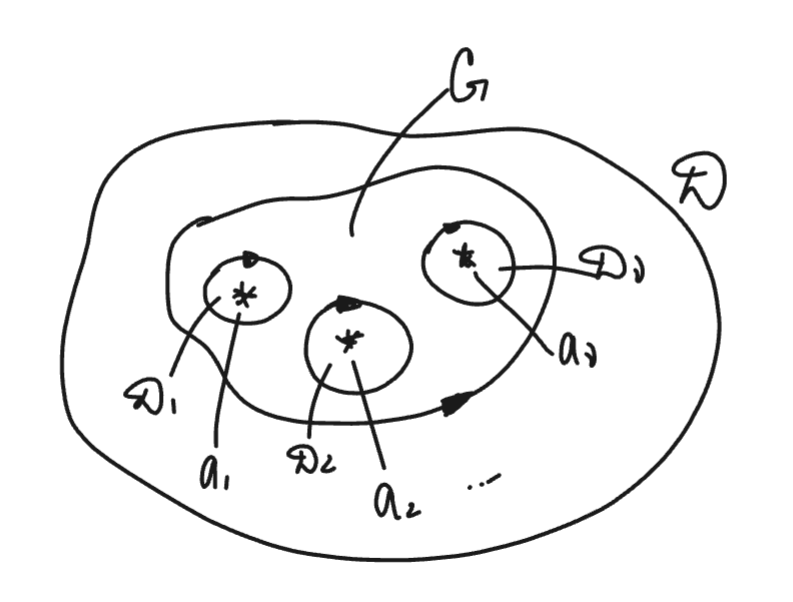
\includegraphics[width=1\linewidth]{answers/img/ans15.png}
    \end{figure}
    Окружности, окружающие $a_1, ..., a_\nu$ не пересекаются и лежат внутри $\gamma G$.\\
    $\tilde{G}=G\backslash (D_1 \cup ...\cup D_\nu), f\in H(\tilde{G})$\\
    $\int\limits_{\gamma \tilde{G}} f(z)dz = 0 \Rightarrow \int\limits_{\gamma G}...+\sum_{j=1}^\nu \int\limits_{-\gamma D_j}...=0 \Rightarrow$\\
    $\Rightarrow \int\limits_{\gamma G}...-\sum_{j=1}^\nu 2\pi i \cdot res\, f(a_j)=0 \Rightarrow \int\limits_{\gamma G}f(z)dz=2\pi i \sum_{j=1}^\nu res\,f(a_j)$.
\end{proof}
\newpage
\section{Характеризация в терминах рядов Лорана изолированной особой точки $\infty$. Вычет в бесконечности.}


\textbf{Точка }$\mathbf{\infty}$ --- \textbf{изолированная особая точка} функции $f$, если:
$$\exists R > 0: \ f\in H(\overset{\circ}{U_{R}}(\infty))$$

Разложение в ряд Лорана в окрестности $\infty$:
$$f(z)=\sum_{n=-\infty}^{+\infty} c_n z^n\text{, обл. сход. содержит } U_R(\infty)$$

Главная часть: $\sum_{n=1}^{+\infty} c_n z^n$

Правильная часть: $\sum_{n=0}^{-\infty} c_n z^n$

Классификация особой точки $\infty$ (характеризация):
\begin{enumerate}
    \item \textbf{Устранимая}, если существует конечный  предел функции в этой точке.
    \item \textbf{Полюс}, если предел функции равен бесконечности в этой точке.
    \item \textbf{Существенно особая}, если не существует предела функции в этой точке.
\end{enumerate}

\textbf{Характеризация устранимой особой точки:}\\
Если точка $\infty \in \overline{\mathbb{C}}$ --- изолированная особая точка функции $f$, то следующие условия эквивалентны:
\begin{enumerate}
    \item $\infty$ --- устранимая особая точка
    \item Лорановское разложение функции $f$ в окрестности точки $\infty$ не содержит главной части. 
    \item Функция $f$ ограничена в окрестности точки $\infty$.
\end{enumerate}

\begin{proof}
    \ \\
    "$2)\to 1)$":\\
    Разложение в ряд Лорана в $\overset{\circ}{U_{\delta}}(\infty):$\\
    $f(z)=\sum_{n=0}^{-\infty} c_n z^n \to c_0$ при $z\to \infty \Rightarrow 1)$\\[2mm]
    "$1) \to 3)$":\\
    $\lim\limits_{z\to \infty}f(z)=A\in\mathbb{C} \Rightarrow f$ -- ограниченная в некоторой окрестности точки $\infty$.\\[2mm]
    "$3) \to 2) $":\\
    $\exists \delta_1 > 0, \ f\in H(\overset{\circ}{U}_{\delta_1}(\infty)) \Rightarrow$ по теореме Лорана\\
    $\Rightarrow f=\sum_{n=-\infty}^{+\infty}c_n z^n$ в $\overset{\circ}{U}_{\delta_1}(\infty).$\\
    Пусть $\delta_1 > 0; f$ ограниченна $M>0$ в $\overset{\circ}{U}_{\delta_1}(\infty), \rho \in (\delta_1, +\infty)\Rightarrow$ по неравенству Коши $\Rightarrow \forall n\in\mathbb{Z}: |c_n|\leq \frac{M}{\rho^n}$\\
    Если $n > 0$ (у главной части степени положительные в $\infty$), то $\frac{M}{\rho^n} \to 0$ при $\rho \to +\infty$. Но $|c_n|$ не зависит от выбора $\rho$. Поэтому $c_n = 0$ при $n > 0 \Rightarrow 2)$.\\[2mm]
\end{proof}

\textbf{Характеризация полюса:}\\
Если точка $a\in \mathbb{C}$ --- изолированная особая точка функции $f$, то следующие условия эквивалентны:
\begin{enumerate}
    \item $\infty$ --- полюс
    \item Главная часть Лорановского разложения функции $f$ в окрестности точки $\infty$ содержит конечное (>0) число слагаемых:
    $$f(z)=\sum_{n=-\infty}^{N} c_n z^n,$$
    где $N>0, c_{N}\neq 0$ 
    \item $f=\frac{1}{\varphi}$, где $\varphi \in H(\infty)$ и $\varphi(\infty) = 0, \ \varphi \not\equiv 0$.
\end{enumerate}

\begin{proof}
    \ \\
    "$2) \to 1)$":\\
    $f(z)=\sum_{n=-\infty}^N c_n z^n=z^N\sum_{n=-N}^\infty c_n (z-a)^{n+N},$\\
    где $\frac{1}{(z-a)^N}\to \infty$ при $z\to a$ и $\sum_{n=-N}^\infty c_n (z-a)^{n+N}$ --- степенной ряд $\Rightarrow c_{-N} \neq 0$.\\[2mm]
    "$1) \to 3)$":\\
    $\varphi(z)=
    \begin{cases}
        \frac{1}{f(z)}\text{, если }z\neq a\\
        0\text{, если }z=a
    \end{cases}
    \text{ --- голоморфнаяв точке }a$\\
    Функция $\frac{1}{f(z)}$ имеет устарнимую особую точку в $a \Rightarrow \frac{1}{f(z)}=\sum_{n=0}^\infty a_n(z-a)^n$\\
    $\lim\limits_{z\to a}\frac{1}{f(z)}=0\Rightarrow a_0 =0$\\[2mm]
    "$3) \to 2)$":
    Пусть $N$ -- такое, что $a_0 = 0 = a_1=...=a_{N-1}, \ a_N \neq 0$.   Тогда $\frac{1}{f(z)}=\sum_{n=N}^\infty a_n(z-a)^n=\varphi(z) \Rightarrow $
    $$\Rightarrow f(z)=\frac{1}{\sum_{n=N}^\infty a_n(z-a)^n}=\frac{1}{(z-a)^N}\cdot \frac{1}{\sum_{n=N}^\infty a_n (z-a)^{n-N}},$$
    где $\sum_{n=N}^\infty a_n (z-a)^{n-N}$ -- голоморфна в точке $a$, равна $a_N \neq 0$;\\
    $\frac{1}{\sum_{n=N}^\infty a_n (z-a)^{n-N}}$ -- голоморфна в окрестности точки $a$.\\
    $\Rightarrow f(z)=\frac{1}{(z-a)^N}\sum_{k=0}^\infty c_k (z-a)^k = \sum_{k=0}^\infty c_k (z-a)^{k-N}=$\\
    $=\sum_{n=-N}^\infty \tilde{c_n}(z-a)^n; \tilde{c_{-N}}=c_0\neq 0$\\[2mm]
\end{proof}

\textbf{Характеризация существенно особой точки:}\\
Изолированная особая точка $a$ функции $f$ является существенно особой
$$\Leftrightarrow$$
Главная часть Лорановского разложения функции $f$ в окрестности точки $a$ имеет бесконечное число слагаемых.\\
\begin{proof}
    \ \\
    Следует из характеризаций устранимой особой точки и вычета.\\[2mm]
\end{proof}


\textbf{Вычетом} функции $f$ в точке $\infty$ называют число:
$$res\, f(\infty) = \frac{1}{2\pi i} \oint\limits_{-\gamma_R}f(z)dz,$$
где $\gamma_R=\{a: |z|=R\}$, $R$ -- такое, что вне $\gamma_R$ нет особых точек, кроме, может быть $\infty$.

\textbf{Теорема о связи вычета в бесконечности с рядом Лорана:}

Если в некоторой выколотой окрестности $\infty$ функция $f$ голоморфна, то:
$$res \, f(\infty) = -c_{-1},$$
где $c_{-1}$ --- коэффициент разложения $f$ в ряд Лорана в окрестности $\infty$.

\begin{proof}
    \ \\
    $res \, f(\infty) =\frac{1}{2\pi i} \oint\limits_{-\gamma_R} f(z)dz = \frac{1}{2\pi i}\sum_{n=-\infty}^{+\infty} \oint\limits_{-\gamma_R}c_n z^n dz =$\\
    $= \frac{1}{2\pi i}c_{-1} \oint\limits_{-\gamma_R} \frac{dz}{z} = -c_{-1}$\\
    Прим.: $ \oint\limits_{-\gamma_R} \frac{dz}{z} = -2\pi i$, т.к. обход по часовой стрелке.
\end{proof}

\newpage
\section{Логарифмический вычет, его вычисление. Приращение (полярного) аргумента вдоль пути. Принцип аргумента. Теорема Руше и ее применение.}

Пусть $f \in H(\mathring{U_r}(a)), a \in \mathbb{C}, r > 0$. Тогда вычет функции $\frac{f'(z)}{f(z)} = \frac{d}{dt}Lnf(z)$ в точке $a$ называют \textbf{логарифмическим вычетом функции $f$ в точке $a$.}\\[2mm]

\textbf{Лемма о логарифмическом вычете в нуле и в полюсе:}\\[2mm]
Логарифмический вычет ф. $f(z)$ в точке $a$ равен:
\begin{enumerate}
    \item порядку нуля $a$, если $a$ -- нуль
    \item порядку полюса $a$, если $a$ -- полюс
\end{enumerate}

\begin{proof}
    \ \\
    1) Пусть $a$ --- нуль порядка $n$ ф-ии $f(z)$, тогда:\\
    $f(z) =a_n(z-a)^n + a_{n+1}(z-a)^{n+1}+...=(z-a)^n\cdot \varphi(z)$, где
    $\varphi(z)$ --- сумма степенного ряда, откуда следует, что $\varphi \in H$\\[2mm]
    $\varphi(a)=c_n\neq0\Rightarrow \frac{f'(z)}{f(z)}=\frac{n(z-a)^{n-1}\cdot \varphi(z)+(z-a)^{n}\varphi'(z)}{(z-a)^n \varphi(z)}=\frac{1}{z-a}\left(n+(z-a)\cdot \frac{\varphi'(z)}{\varphi(z)}\right) \Rightarrow a$ --- полюс 1-ого порядка функции $\frac{f'}{f} \Rightarrow C_{-1}=n$, т.к. $\frac{n}{z-a}$ --- главная часть.\\[2mm]
    2) Пусть $a$ --- полюс порядка $p$, тогда по теореме о полюсе $a$ --- нуль порядка $p$ функции $\frac{1}{f(z)}=g(z)$.\\
    $\frac{f'(z)}{f(z)} = -\frac{d}{dz} Ln\frac{1}{f(z)}$\\
    Тогда логарифмический вычет функции $g$ в точке $a$ равен $p$, а функции $f$ в точке $a$ равен $-p$.
\end{proof}
\ \\

\textbf{Теорема о логарифмическом вычете:}\\[2mm]
Пусть $f$ мероморфна в области $D \subset \mathbb{C}, G \cup \partial G \subset D, \partial G$ не содержит ни нулей, ни полюсов функции $f$, $N$ и $P$ -- количество нулей и полюсов с учетом их порядков функции $f$ в $G$.\\
Тогда $\frac{1}{2\pi i}$ \(\int\limits_{\partial G} \frac{f'(z)}{f(z)}\, dz\) $= N - P$ (обход $\partial G$ против часовой стрелки),\\
где \(\int\limits_{\partial G} \frac{f'(z)}{f(z)}\, dz\) -- логарифмический вычет функции $f$ вдоль кривой $\partial G$.

\begin{proof}
    \ \\
    Особые точки $\frac{f'(z)}{f(z)}$ в области $G$:
    \begin{enumerate}
        \item полюса $a_1, .., a_l$ с порядками $p_1, ..., p_l$
        \item нули $b_1, .., b_m$ с порядками $n_1, ..., n_m$
    \end{enumerate}
    Тогда по лемме о логарифмическом вычете $res\frac{f'}{f}(a_j)=-p_j$, $res\frac{f'}{f}(b_s)=n_s$\\
    По теореме Коши:
    $$\frac{1}{2\pi i}\int\limits_{\partial G} \frac{f'(z)}{f(z)}dz =\frac{1}{2\pi i}\cdot 2\pi i \left(\sum_{j=1}^l res\frac{f'}{f} (a_j) + \sum_{s=1}^m res \frac{f'}{f)}(b_s)\right) =$$
    $$= - \sum_{j=1}^l p_j +\sum_{s=1}^m n_s = N-P$$
\end{proof}


$\Delta_{\gamma}arg f = 2\pi k$, k -- количество обходов точки $О$ функцией f(z), $z \in \gamma$, с учетом направления.

\begin{figure}[h]
    \centering
    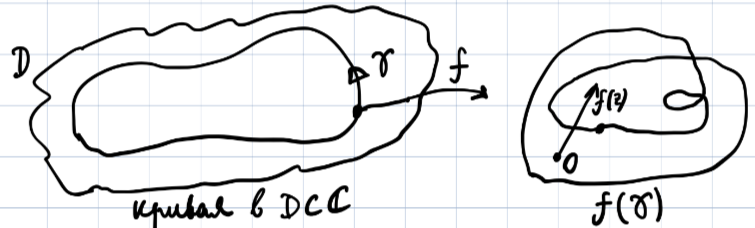
\includegraphics[width=0.5\linewidth]{answers/img/image1.png}
    \label{fig:enter-label}
\end{figure}

\textbf{Принцип аргумента}. Пусть f мераморфна в $ D \subset \mathbb{C}, \, G \cup \partial G \subset D, \, \partial G$ не содержит ни нулей, ни полюсов f. Тогда 

$N-P = \frac{1}{2 \pi}\Delta_{\partial G}arg f$.

\begin{proof}
    \ \\
    Пусть $\partial G: \ z=z(t), \ t\in[\alpha, \beta]$,
    $\Phi(t)=\ln f(z(t))$, где $\ln f$ непрерывно меняется при росте $t$ от $\alpha$ до $\beta$. Тогда $\Phi'(t)=\frac{f'(z(t))}{f(z(t))}\cdot z'(t)$ и поэтомy
    $$\int\limits_{\partial G}\frac{f'}{f}dz = \int\limits_{\alpha}^{\beta} \frac{f'(z(t))}{f(z(t))}z'(t)dt=\Phi(\beta) - \Phi(\alpha) = $$
    $$= \ln f(z(\beta))-\ln f(z(\alpha)) = \ln |f(z(\beta))| + i \, arg \, f(z(\beta))-\ln |f(z(\alpha))| -$$
    $$ -i\cdot arg\, f(z(\alpha))=i\Delta_{\partial G}arg \, f \Rightarrow \text{ (по т. о логар.выч.): }$$
    $$N-P==\frac{1}{2\pi i}\int\limits_{\partial G} \frac{f'(z)}{f(z)}dt=\frac{i\Delta_{\partial G}arg\,f}{2\pi i}$$
\end{proof}


\textbf{Теорема Руше:}\\
Пусть $f,g \in H(G \cup \partial G) \ \textrm{и} \ \forall z \in \partial G: |f(z)| > |g(z)|$. \\
Тогда функции f и f+g имеют одинаковое количество нулей в G.\\[2mm]

\begin{proof}
    \ \\
    $\forall z \in \partial G: |f(z)|>|g(z)|\geq 0$\\
    $|(f+g)(z)| \geq |f(z)| - |g(z)| > 0$\\
    Отсюда следует, что функция $f$ и $f+g$ не имеют нулей на $\partial G$.\\
    По принципу аргумента $\Delta_{\partial G}arg\, (f+g) = N_{f+g}$ (количество нулей функции $f+g$ в $G$).\\
    С другой стороны:\\
    $\Delta_{\partial G} arg\, f(1+\frac{g}{f})=\Delta_{\partial G} arg\, f+\Delta_{\partial G}(1+\frac{g}{f})=N_f,$\\
    так как $\forall z \in \partial G: \ \left|\frac{g}{f}\right|<1.$

    
\end{proof}
\textbf{Применение:}\\
Найти число корней уравнения $z^8-4z^5+z^2-1=0$ в области $|z|<1$.\\
На границе области $|z|=1$, тогда т.к. $|z^8+z^2-1|\leq |z|^8+|z|^2+|-1|=3 < |-4z^5|=4$ и уравнение $-4z^5=0$ имеет 5 корней в этой области, то исходное уравнение также иммеет 5 корней в этой области.

\newpage
\section{Теорема о среднем и принцип максимума модуля. Принцип сохранения области.}

\textbf{Теорема о среднем:}\\[2mm]
Пусть $f \in H(D), z_0 \in D, \partial U_{\rho}(z_0)\subset D$\\
Тогда $f(z_0) = \frac{1}{2\pi} \int\limits_{0}^{2\pi} f(z_0+\rho e^{it})dt$

\begin{proof}
    \ \\
    По интегральной формуле Коши:
    $$f(z_0)=\frac{1}{2\pi i}\int\limits_{\partial U_{\rho}(z_0)}\frac{f(z)}{z-z_0}dz = \frac{1}{2\pi i} \int\limits_{0}^{2\pi}\frac{f(z_0+\rho e^{it})}{\rho e^{it}}i\rho e^{it}dt=$$
    $$=\frac{1}{2\pi}\int\limits_0^{2\pi}f(z_0+\rho e^{it})dt$$
    Параметр $\partial U_{\rho}(z_0): \ z=z_0+\rho e^{it}: \ t\in[0; 2\pi], z'=i\rho e^{it}$
\end{proof}

\textbf{Принцип сохранения области:}\\[2mm]
Функция $f$ голоморфна в области $D$ и $f\neq const$
$$\Rightarrow$$
Образ $f(D)$ есть область

% \begin{proof}
%     \ \\
%     Нужно показать, что множество $D^*$ связно и открыто.\\
%     1) Пусть $w_1, w_2$ --- две произвольные точки $D^*$, а $z_1, z_2$ --- их прообразы.\\
%     Так как множество $D$ линейно связно, то существует путь $\gamma: [\alpha; \beta]\rightarrow D$, связывающий точки $z_1, z_2$. В силу непрерывности функции $f$ образ $\gamma^*=f\circ \gamma$ будет путем, связывающим точки $w_1, w_2$. Таким образом $D^*$ --- линейно связно.\\[2mm]
%     2) Пусть $w_0$ произвольная точка $D^*$ и $z_0$ --- один из ее прообразов в $D$. Так как $D$ открыто, то сущестует круг $\{|z-z_0|\leq r\}\subset D$. \\
%     Будем уменьшать $r$ пока круг не перестанет содержать других точек, в которых функция $f$ равна $w_0$ (это возможно, т.к. она не постоянная).\\
%     Обозначим $\gamma=\{|z-z_0|=r\}$ границу этого круга и
%     $$\mu=\underset{x\in \gamma}{\min}|f(x)-w_0|, \ \mu>0$$
%     Если бы $\mu =0$, то на $\gamma$ существовала бы точка, в которой функция $f$ равна $w_0$.\\[2mm]
%     Теперь докажем, что $\{|w-w_0|<\mu\} \subset D^*$.\\
%     Пусть $w_1$ --- произвольная точка этого круга, то есть $|w_1-w_0|<\mu$. Тогда:\\
%     $f(z)-w_1=f(z)-w_0+(w_0-w_1)$.\\
%     Так как на $\gamma$ в силу выбора $\mu$ имеем $|f(z)-w_0|\geq \mu$, то по теорему Руше функция $f(z)-w_1$ имеет внутри $\gamma$ столько же нулей, сколько и $d(z)-w_0$, то есть по крайней мере один нуль $z_0$, а значит функция $f$ внутри $\gamma$ принимает значение $w_1$, то есть $w_1 \in D^*$. В силу произвольности выбора $w_1$ весь круг лежит в $D^*$, а значит оно является открытым множеством.
% \end{proof}


\textbf{Принцип максимума модуля:}\\[2mm]
Модуль голоморфной функции не может достигать строгого локального максимума внутри области.\\[2mm]
\begin{proof}
    \ \\
    Пусть функция достигает максимума в некоторой точке $z_0$.\\
    Воспользуемся принципом сохранения области. Если $f\neq const$, то она преобразует $z_0$ в точку $w_0$ области $D^*$. \\
    Существует круг $\{|w-w_0|<\mu\}\subset D^*$, а в нем найдется точка $w_1$ такакя, что  $|w_1|> |w_0|$. Значение $w_1$ принимается функцией $f$ в некоторой окрестности точки $z_0$, а это противоречит тому, что $|f|$ достигает максимума в этой точке.
\end{proof}

\newpage
\section{Основные теоремы и приложения теории конформных отображений. Теорема Римана, принцип симметрии Римана-Шварца, принцип соответствия границ с обратным принципом соответствия границ.}

\textbf{Основные теоремы и приложения конформных отображения:}\\
\begin{enumerate}
\item \textbf{Теорема Римана} (о возможности конформного и взаимно однозначного отображения одной односвязной области на другую)\\
Пусть $D$ -- односвязная область в $\overline{\mathbb{C}}$, граница которой содержит не менее двух точек. Тогда: 
\begin{enumerate}
    \item $\exists$ голоморфная в $D$ функция $w=f(z)$, которая отображает $D$ конформно и однозначно на единственный круг $G: |w|<1$;
    \item эту функцию можно выбрать так, что $f(z_0)=w_0, \, \textrm{arg} f'(z_0)=\alpha$, где $Z_0 \in D, \, w_0 \in G$ -- заданные точки, $\alpha$ -- заданное действительное число.
\end{enumerate}
Функция $f$, удовлетворяющая 1. и 2. единственная.\\[2mm]

\item \textbf{Принцип симметрии Римана-Шварца}\\
Пусть $D_1$ -- односвязная область, лежащая в верхней полуплоскости $Im z>0$, граница Г$_1$, которая содержит интервал $\gamma$ действительной оси $Im z =0$, область $D_2$ симметрична $D_1$ относительно действительной оси, функция $f(z)$ непрерывна на $D_1$, Г$_1$, голоморфна на $D_1$ и принимает действительные занчения на $\gamma$. Тогда функция $f$ может голоморфно продолжить в область $D_1 \cup \gamma \cup D_2$ по формуле:
\begin{equation}
    f(z) = \begin{cases}
        f_1(z), & \textrm{если} z \in D_1 \cup \gamma, \\
        \overline{f_1(\overline{z})}, & \textrm{если} z \in D_2.
    \end{cases}
\end{equation}

\begin{figure}[h]
    \centering
    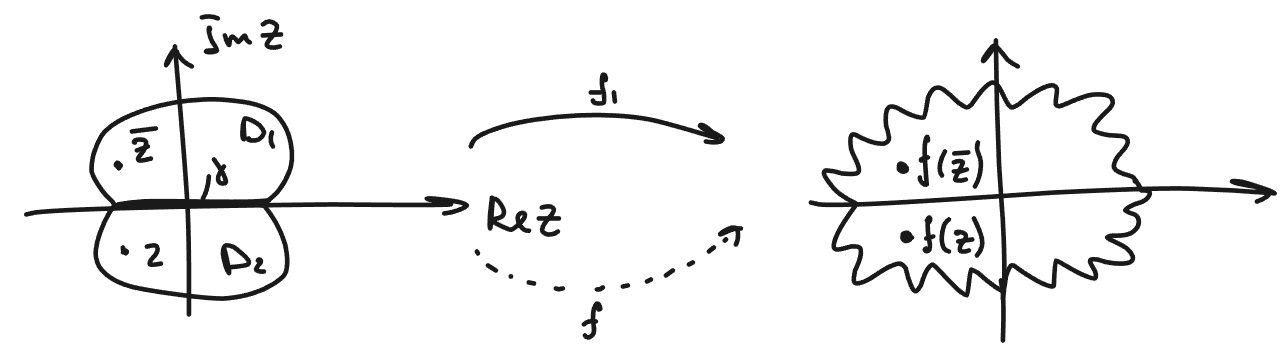
\includegraphics[width=1\linewidth]{answers/img/14_2.png}
\end{figure}

\item \textbf{Принцип соответствия границ}\\
Пусть Г и Г* -- простые контуры, $D$ и $D \ast$ -- односвязные области, ограниченные Г и Г* соответственно, функция $f(z)$ однолистно и конформно отображает $D$ на $D \ast$. Тогда 
\begin{enumerate}
    \item $f(z)$ имеет непрерывное продолжение $\overline{f}$ на Г, то есть $\overline{f}: \overline{D}=D \cup \textrm{Г} \rightarrow \mathbb{C}$ -- непрерывна и $\overline{f}|_D=f$
    \item $\overline{f}$ отображает Г на Г* взаимно однозначно, причемположительному обходу Г соответствует положительный обход Г*.\\[2mm]
\end{enumerate}

\item \textbf{Обратный принцип соответствия границ}\\
Пусть $D$ -- односвязная область в $\mathbb{C}$, ограниченная кусочно-гладким контуром Г. $\overline{D}=D \cup \textrm{Г}, \, f \in H(D),$ функция $f(z)$ отображает контур Г взаимно однозначно на простой кусочно-гладкий контур Г*.\\
Тогда $f(z)$ отображает $D$ конформно и однозначно на область $D \ast$, ограниченную контуром Г*, причем положительному обходу Г соответствует положительный обход Г*.


\end{enumerate}
\newpage 
\section{Вычисление несобственных интегралов с использование вычетов. Лемма Жордана и теорема о вычислении несобственного интеграла от рациональной функции с помощью вычетов.}

\textbf{Лемма Жордана:}\\[2mm]
Пусть  $f(z)$ --- непрерывная функция в $\{Im\,z \geq 0\}$ за исключением изолированного множества точек;

$\gamma_{R} =\{z\in\mathbf{C}: \, |z|=R, \, Im\,z\geq 0\}$;

$M(R)=\underset{z\in \gamma_{R}}{\max}|f(z)|, \, M(R) \rightarrow 0$ при $R\rightarrow \infty$;\\[2mm]
Тогда $\forall \lambda > 0 \, \int\limits_{\gamma_{R}} f(z)e^{i\lambda z}dz\rightarrow 0$\\[4mm]

\textbf{Теорема о вычислении несобственного интеграла от рациональной функции с помощью вычетов:}\\[2mm]
Пусть  $f(x)=\frac{P_m(x)}{Q_n(x)}$, где $P_m(x), Q_n(x)$ -- многочлены степени $m$ и $n$ соответственно, $n\geq m+2$;

$Q_n(x)\neq 0$ при $x \in \mathbb{R}$ (не имеет действительных корней);\\[2mm]
Тогда $\int\limits_{-\infty}^{+\infty}f(x)dx=2\pi i \sum_{j=1}^k res\,f(z_j)$, 

где $z_1, ...,z_k$ -- все полюса $f$ в области $Im\,z >0$\\[2mm]

\begin{proof}
    \ \\
    \begin{figure}[h]
        \centering
        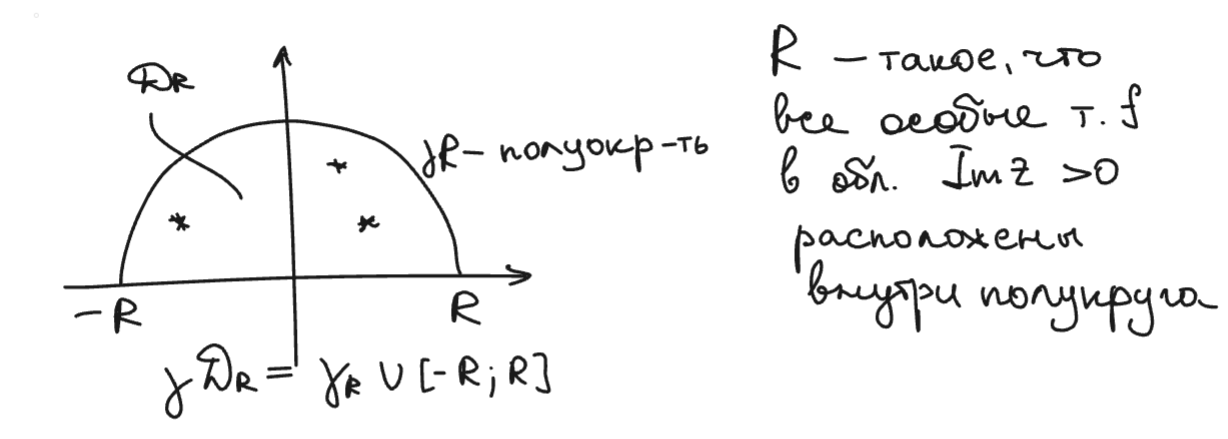
\includegraphics[width=1\linewidth]{answers/img/ans21.png}
    \end{figure}\\[2mm]

    Так как $f$ непрерывна на компакте $\gamma_R$, то $\exists \underset{z\in \gamma_R}{\max} |f(z)|$.\\[2mm]
    $\max\frac{|P_m(z)|}{|Q_n(z)|}=\underset{|z|=R, Im\,z\geq0}{\max} \frac{|d_mz^m+...|}{|a_nz^n+...|} \sim{} \underset{|z|=R, Im\,z\geq0}{\max} \frac{|b_m||z|^m}{|a_n||z|^n}= $\\[2mm]
    $=\underset{|z|=R}{\max}\frac{|b_m|}{|a_n|}\cdot\frac{1}{|z|^{n-m}}\sim{} \frac{|b_m|}{|a_n|}\cdot \frac{1}{R^{n-m}}$ при $R\to \infty$\\[2mm]
    Пусть $L(\gamma_R)$ -- длина $\gamma_R$. Тогда:\\[2mm]
    $\left|\int\limits_{\gamma_R}f(z)dz\right|\leq \underset{a\in\gamma_R}{\max}|f(z)|\cdot L(\gamma_R)\sim c\frac{1}{R^{n-m}}\pi R = \frac{c\pi}{R^{n-m-1}}\to 0$ при $R\to \infty, n-m-1>0$\\[2mm]
    Откуда следует, что $\left|\int\limits_{\gamma_R} f(z)dz\right| \to 0$ при $R\to \infty$.\\[2mm]
    По теореме Коши: $\oint\limits_{\gamma D_R}f(z)dz = 2\pi i \sum\limits_{j=1}^k res\, f(z_j)$ не зависит от $R$, при $R\to \infty:$\\[2mm]
    $\oint\limits_{\gamma D_R}f(z)dz = \int\limits_{\gamma_R}f(z)dz + \int\limits_{-R}^R f(x)dx \to 0+\int\limits_{-\infty}^{-\infty}f(x)dx$.
\end{proof}


\newpage
\textbf{Пример вычисления несобственного интеграла от тригонометрических функций:}\\
Вычислить интеграл $\int\limits_{-\infty}^{+\infty} \frac{x\cos x dx}{x^2-2x+10}$\\
Функция $f(z)=\frac{ze^{iz}}{z^2-2z+10}$ удовлетворяет условиями леммы Жордана. Здесь $t=1$ и $F(z)=\frac{z}{z^2-2z+10}$. Особыми точками функции $f(z)$ являются полюсы первого порядка $z=1\pm 3i$. В верхней полуплоскости иммется единственная особая точка $z=1+3i$. Вычислим относительно этой точки вычет функции $f(z)$:
$$res\, f(1+3i) = \frac{ze^{iz}}{(z^2-2z+10)'}=\frac{(1+3i)e^{-3+i}}{6i}$$
Следовательно, $\int\limits_{-\infty}^{+\infty} \frac{xe^{ix}dx}{x^2-2x+10}=2\pi i \frac{(1+3i)e^{-3+i}}{6i} = \frac{\pi}{3}e^{-3}(1+3i)(\cos 1+i\sin 1)=\frac{\pi}{3} e^{-3}(\cos 1 - 3\sin 1)+i\frac{\pi}{3}e^{-3}(3\cos 1+\sin 1).$\\
Сравнивая в обеисх частях этого равенства действительные и мнимые части с учитывая, что $$\int\limits_{-\infty}^{+\infty}\frac{xe^{ix}dx}{x^2-2x+10}=\int\limits_{-\infty}^{+\infty}\frac{x\cos x\, dx}{x^2-2x+10}+i\int\limits_{-\infty}^{+\infty}\frac{x\sin x\, dx}{x^2-2x+10}$$ 
получим $$\int\limits_{-\infty}^{+\infty}\frac{x\cos x\, dx}{x^2-2x+10} = \frac{\pi}{3}e^{-3}(\cos 1-3\sin 1),$$
$$\int\limits_{-\infty}^{+\infty}\frac{x\sin x\, dx}{x^2-2x+10} = \frac{\pi}{3}e^{-3}(3\cos 1+\sin 1),$$

\newpage
\section{Определение преобразования Лапласа. Теорема о существовании изображения. Поведение изображения в бесконечно удаленной точке. Изображение элементарных функций (единичная функция Хевисайда, показательная и степенная функции). Теорема обращения.}


Пусть $f(t)$ --- функция, $t \in \mathbb{R}$\\
\textbf{Преобразование Лапласа} функции $f$ --- это $$F(p)=\int\limits_{0}^{+\infty}f(t)e^{-pt}dt, \in \mathbb{C}$$
Обозначение: $F(p)\risingdotseq f(t), f(t)\fallingdotseq F(p)$


\newpage
\section{Основные свойства преобразования Лапласа. Теоремы линейности, подобия, затухания, запаздывания, опережения, дифференцирования и интегрирования оригинала, дифференцирования и интегрирования изображения. Свертка двух функций. Теорема умножения изображений. Доказать теоремы затухания и дифференцирования оригинала, сформулировать остальные теоремы.}


\newpage
\section{Три теоремы разложения. Доказать теоремы подобия и запаздывания.}


\end{document}
